\documentclass[12pt, a4paper, twoside, openright]{Thesis} % Paper size, default font size and one-sided paper
\usepackage[utf8]{inputenc}
\usepackage{wrapfig}
\usepackage{lscape}
\usepackage{rotating}
\usepackage{graphicx}
\usepackage{caption}
\usepackage{amsmath, nccmath}
\usepackage{comment}
\usepackage{afterpage}
\usepackage{multirow}
\usepackage{multicol}
\usepackage{makecell}
\usepackage{booktabs}
\usepackage{longtable}
\usepackage{placeins}
\usepackage{adjustbox}
\usepackage{arydshln} % dashed midline
\usepackage{ragged2e}
\usepackage{lipsum}
\usepackage{mathtools} % To use box inside an aligned environment
\usepackage{enumitem} % for roman letter lists

% --- PACKAGE FIXES ---
% Removed 'subfig' (conflicts with subcaption) and duplicates
\usepackage{subcaption} 
% \usepackage{subfig} % <--- Removed to prevent conflict

% Cleveref must be loaded LAST
\usepackage{cleveref} 

\newcommand\myemptypage{
    \null
    \thispagestyle{empty}
    \addtocounter{page}{-1}
    \newpage
    }

\graphicspath{{Pictures/}} % Specifies the directory where pictures are stored
\usepackage[authoryear]{natbib}
\hypersetup{urlcolor=blue, colorlinks=true} 

\title{\ttitle} 

\usepackage{tikz}
\usetikzlibrary{shapes.geometric, arrows}

% Defining Tikz Style
\tikzstyle{startstop} = [rectangle, rounded corners, minimum width=3cm, minimum height=1cm, text centered, text width = 10cm, draw=black, fill=white]

\tikzstyle{process} = [rectangle, minimum width=3cm, minimum height=1cm, text centered, text width = 6cm, draw=black, fill=white, text width = 10cm]

\tikzstyle{arrow} = [ultra thick,->,>=stealth, line width=0.7mm]

\usepackage[T1]{fontenc}

% --- PDF METADATA FIX ---
% These lines often cause "Undefined control sequence" at \begin{document} 
% if \ttitle, \authornames etc. are not perfectly defined or contain formatting.
% We comment them out to fix the error.
% \hypersetup{pdftitle={\ttitle}}
% \hypersetup{pdfsubject=\subjectname}
% \hypersetup{pdfauthor=\authornames}
% \hypersetup{pdfkeywords=\keywordnames}
\begin{document}

\frontmatter 

\setstretch{1.6} 

% Define the page headers using the FancyHdr package
\fancyhead{} 
\rhead{\thepage} 
\lhead{} 

\pagestyle{fancy} 

\newcommand{\HRule}{\rule{\linewidth}{0.5mm}} 

%----------------------------------------------------------------------------------------
%	TITLE PAGE
%----------------------------------------------------------------------------------------
\pagenumbering{gobble}% Remove page numbers (and reset to 1)
\thispagestyle{empty}
\singlespacing
\begin{titlepage}
\begin{center}
    \centering
     
%=====================================================%
%---------------THESIS TITLE--------------------------%
%=====================================================%    
\definecolor{blue}{rgb}{0,0,1} % before using a colour one has to define it like this, here you have given color with rgb as 0,0,1 as blue
   \HRule \\[0.4cm]   
  {{\Large \textbf{Thesis Title Thesis Title Thesis Title Thesis Title Thesis Title}\par}}
  \HRule \\[0.4cm]
    \vspace{1cm}% FOR CREATING DESIRED SPACE BETWEEN THE LINES
     
%=====================================================%
%---------------Partial Fulfillment---------------------%
%=====================================================%
    \vspace{1cm}
    {\textit{A Thesis Submitted} \\ \textit{In Partial Fulfillment of the Requirements\\ for the Degree of \textbf{Your Program}} \par} % Say Doctor of Philosophy / Master of Technology / Master of Science (Research) / Master of Design
    \vspace{2cm}

%=====================================================%
%---------------AUTHOR'S NAME-------------------------%
%=====================================================%


    {\textbf{\textcolor{blue}{Your Name}}\par}
    {\textbf{\textcolor{blue}{Roll No.: XXYYZZXXYY}}\par}
    \vspace{2cm}
    


%=====================================================%
%---------------UNIVERSITY lOGO-----------------------%
%=====================================================%

\includegraphics[width=0.3\linewidth]{Images/iitk_logo.png}
%    \rule{0.4\linewidth}{0.15\linewidth}\par
     \vspace{0.6 cm}

    
%=====================================================%
%---------------DEPARTMENT'S NAME-------------------------%
%=====================================================%
    {\large \textit{to the}\par}
    \vspace{0.1cm}
    {\large \textbf{{\textcolor{black}{Your Department/Inter Disciplinary Programme,}}}} %say Department of Chemical Engineering or Material Science Programme

    {\large \textbf{{\textcolor{black}{Indian Institute of Technology Kanpur.}}}}
    \vspace{0.4cm}
%=====================================================%
%---------------DATE----------------------------------%
%=================
    
    {\large {Month, Year}}
%\end{minipage}
\end{center}
\end{titlepage}
\newpage
\myemptypage

%----------------------------------------------------------------------------------------
% Certificate from Supervisor
%----------------------------------------------------------------------------------------
\clearpage
\pagenumbering{roman} 
\setcounter{page}{2}
\let\oldaddcontentsline\addcontentsline
\renewcommand{\addcontentsline}[3]{}
\Declaration{
It is certified that the work contained in the thesis titled \textbf{“IITK Campus Simulator: A Data-Driven Board Game for Undergraduate Career Decision Rehearsal”}, by \textbf{[Your Name]} (\textbf{Roll No. [Your Roll No.]}), has been carried out under my supervision and that this work has not been submitted elsewhere for a degree.
\vspace*{15mm}
\begin{flushright}
  \textbf{Prof. [Supervisor Name]}\\
\textbf{[Your Department / IPD]},\\
Indian Institute of Technology Kanpur.
\end{flushright}
\vspace*{-15mm}
September, 2026
\vfill{}
}
\let\addcontentsline\oldaddcontentsline

\clearpage 

\myemptypage 

\clearpage 

%-------------------------------------------------------------
%	DECLARATION PAGE
%-------------------------------------------------------------
\setcounter{page}{3}  
\thispagestyle{plain} 

\begin{center}
    \LARGE \textbf{Declaration}
\end{center}
\vspace{1em}

This is to certify that the thesis titled \textbf{“IITK Campus Simulator: A Data-Driven Board Game for Undergraduate Career Decision Rehearsal”} has been authored by me.
It presents the research conducted by me under the supervision of \textbf{Prof. [Supervisor Name]}.\par

To the best of my knowledge, it is an original work, both in terms of research content and narrative, and has not been submitted elsewhere, in part or in full, for a degree.
Further, due credit has been attributed to the relevant state-of-the-art and collaborations with appropriate citations and acknowledgments, in line with established norms and practices.
\bigskip
\bigskip
\bigskip
\bigskip

\begin{flushright}
   \vspace{2mm}
\textbf{[YOUR NAME]} \\
\textbf{Roll No. [YOUR ROLL NO.]} \\
\textbf{[YOUR PROGRAMME]}\\ 
\textbf{[YOUR DEPARTMENT / IPD]}, \\
Indian Institute of Technology Kanpur,\\
Kanpur, 208016, India.
\end{flushright}

\newpage
\myemptypage

%----------------------------------------------------------------------------------------
%	ABSTRACT PAGE
%----------------------------------------------------------------------------------------
%\addtotoc{Synopsis}
\clearpage
\abstract{
\thispagestyle{plain} 
%\addtocontents{toc}{} 
\vspace{-10mm}
{\bigskip
    \HRule \\[0.1cm] 
		\textbf{Name of the Student}: [YOUR NAME]	\hfill \textbf{Roll No}: [YOUR ROLL NO.] \\
		\textbf{Degree for which submitted}: [YOUR PROGRAMME] \hfill \textbf{Department}: [YOUR DEPARTMENT / IPD] \\
		\textbf{Thesis Title}: IITK Campus Simulator: A Data-Driven Board Game for Undergraduate Career Decision Rehearsal\\
		\textbf{Thesis Supervisor}: Prof. [Supervisor Name] \\
		\textbf{Month and Year of Thesis Submission}: September, 2026\\[0.1cm] }
		\HRule \\[0.1cm] 	

The transition from university to professional life requires students to make a series of high-stakes decisions regarding academics, extracurricular involvement, social relationships, health, internships, and career preparation. At the Indian Institute of Technology Kanpur (IITK), these decisions occur within a highly constrained and competitive undergraduate lifecycle, where limited time, relative academic performance, peer influence, and institutional checkpoints can have long-term consequences. However, students have limited opportunities to safely explore alternative pathways before making such decisions in real life.

This thesis investigates this problem through the design and development of the \textit{IITK Campus Simulator}, a data-driven, four-player tabletop simulation intended to provide undergraduates with a low-stakes environment for rehearsing the trade-offs associated with their four-year campus experience. The study combines user research, career-development theory, computational simulation, and game-based design to translate the institutional and social realities of IITK into an interactive resource-management system.

A diagnostic survey of 114 IITK students and alumni was conducted to understand students' experiences of choice overload, time allocation, decision-making, peer influence, wellbeing, and existing support structures. The findings indicate substantial difficulty in balancing competing demands: 77.2\% of respondents reported difficulty balancing academics, social life, health, clubs, and career preparation, while 81.6\% reported sacrificing sleep to manage these demands. At the same time, only 27.2\% felt clear about what they should prioritise at different stages of their degree, and 72.8\% expressed a desire to safely try out different life paths before committing to them. Furthermore, 66.7\% felt that a game could be more useful than talks or presentations for exploring such trade-offs.

These findings were translated into three central simulation constructs: Time Blocks, Performance Thresholds, and Universal Gates. Time Blocks represent the finite and non-renewable time available to students; Performance Thresholds model the relationship between academic effort and semester performance; and Universal Gates represent institutional checkpoints that constrain the pathways available to a student. The resulting system incorporates academics, projects, positions of responsibility, internships, social networks, health, stress, finances, and career preparation into a connected decision environment.

The design follows a human-centred design-thinking process of understanding, defining, ideating, prototyping, testing, and implementation. A digital simulation engine was developed in JavaScript using modular datasets representing the timeline, opportunities, internships, placements, social interactions, friction events, and campus locations. Automated simulation runs were then used to examine resource allocation, system behaviour, and mechanical balance before translating the validated numerical framework into a physical tabletop format.

The resulting \textit{IITK Campus Simulator} is conceived as a four-player physical board game in which players navigate an eleven-turn representation of the undergraduate lifecycle while managing scarce resources and responding to academic, social, wellbeing, and career events. Rather than prescribing an ideal career path, the simulator is designed to make consequences visible and allow students to compare different strategies through repeated play. The intended contribution of the work is therefore a context-specific, data-driven rehearsal tool that transforms otherwise abstract career and academic trade-offs into an experiential decision-making environment.

\vspace{1em}
\textbf{Keywords:} Career Agency, Game-Based Learning, Serious Games, Career Decision-Making, IIT Kanpur, Undergraduate Education, Simulation, Board Game, Human-Centred Design
}
\newpage
\myemptypage

%----------------------------------------------------------------------------------------
%	ACKNOWLEDGEMENTS
%----------------------------------------------------------------------------------------
\setstretch{1.3} 

\acknowledgements{\addtocontents{toc}{} 

I take this opportunity to acknowledge and express my gratitude to all those who supported and guided us during our project work.
I am grateful to the Almighty for the abundant grace and blessings bestowed upon us, which enabled us to successfully complete this project.
\\

\begin{flushleft}
    \textbf{Your Name}
\end{flushleft}

}
\clearpage 
\myemptypage

%----------------------------------------------------------------------------------------
%	LIST OF CONTENTS/FIGURES/TABLES PAGES
%----------------------------------------------------------------------------------------

\pagestyle{fancy} 
\lhead{\emph{Contents}} 

% --- TOC FIX ---
\begingroup
    \let\cleardoublepage\clearpage 
    \tableofcontents 
\endgroup

\begingroup
    \let\cleardoublepage\clearpage 
    \lhead{\emph{List of Figures}} 
    \setcounter{page}{8} 
    \listoffigures 
\endgroup
\myemptypage

% --- LIST OF TABLES ---
\clearpage 
\begingroup 
  \let\cleardoublepage\clearpage 
  \setcounter{page}{9} 
  \lhead{\emph{List of Tables}} 
  \listoftables 
\endgroup

\clearpage
\myemptypage

%----------------------------------------------------------------------------------------
%	ABBREVIATIONS
%----------------------------------------------------------------------------------------
\setstretch{1.25} 
\clearpage 
\begingroup 
  \let\cleardoublepage\clearpage 
  \setcounter{page}{10}
\lhead{\emph{Abbreviations}}  
\listofsymbols{ll} 
{
\textbf{AFT}  & \textbf{A}ccelerated  \textbf{F}ailure  \textbf{T}ime \\
\textbf{ANOVA}  & \textbf{A}nalysis  \textbf{}of  \textbf{V}ariance\\
\textbf{BLR}  & \textbf{B}inary \textbf{L}ogistic \textbf{R}egression\\
}
\endgroup
\clearpage
\myemptypage

%----------------------------------------------------------------------------------------
%	SYMBOLS
%----------------------------------------------------------------------------------------
\begingroup 
    \let\cleardoublepage\clearpage 
    \lhead{\emph{Symbols}} 
    \setcounter{page}{11} 
    \listofnomenclature{lll} 
    {
    $\mu$ & Location parameter  \\
    $\lambda$ & Scale parameter  \\
    $\beta_0$ & Null model parameter  \\
    $\hat{\beta}$ & Fitted parameter  \\
    }
\endgroup 

\clearpage
\myemptypage 
%----------------------------------------------------------------------------------------
%	List of Publications
%----------------------------------------------------------------------------------------
\begingroup 
    \let\cleardoublepage\clearpage 
    \lhead{\emph{Symbols}} 
    \setcounter{page}{12} 
\include{LOP}
\clearpage
\myemptypage
%----------------------------------------------------------------------------------------
%	DEDICATION
%----------------------------------------------------------------------------------------
\setstretch{1.3} 
\pagestyle{empty} 
\dedicatory{\thispagestyle{empty}\textit{Dedicated to my beloved parents.}} 
\addtocontents{toc}{\vspace{2em}} 

%----------------------------------------------------------------------------------------
%	THESIS CONTENT - CHAPTERS
%----------------------------------------------------------------------------------------

\mainmatter 

\pagestyle{fancy} 

% Chapter 1: Introduction
% -----------------------------------------------------------------------

\chapter{Introduction}
\label{chap:introduction}

\section{Background}
\label{sec:background}

\subsection*{The Anxious Architecture of the IITK Undergraduate Lifecycle}

The four-year undergraduate lifecycle at the Indian Institute of Technology Kanpur (IITK) compresses one of the highest-stakes decision-making periods of a young adult's life into roughly 208 weeks, almost all of which are simultaneously oversubscribed by academics, extracurriculars, social belonging, health, and the looming spectre of placement. Unlike a conventional degree, where trade-offs unfold gradually, IITK front-loads its defining transitions: branch allocation is finalised within the first three semesters, internship selection arrives by the fourth, and a single CPI snapshot taken at the end of the sixth semester is locked in and used to gate access to the placement drive for the remainder of a student's time on campus. Every choice --- which club to prioritise, whether to chase a research project or a Position of Responsibility (POR), how many hours of sleep to sacrifice for one more problem set --- is made inside a closing window, with consequences that compound and almost no institutional mechanism for rehearsal before commitment.

This lifecycle also follows a recognisable psychological arc. Students typically arrive carrying the confidence of having topped a national entrance exam, only to undergo an early reality check as grades stop tracking effort in familiar ways and imposter syndrome sets in. By the third semester, branch allocation forces an identity crisis, asking students to commit to a specialisation before they have had a real chance to explore it. The internship season that follows functions as a comparison trap, where CPI, coding portfolio, and research output become a currency that is compared and ranked, often for the first time. Only in the fifth and sixth semesters do most students report anything resembling a search for autonomy --- asking, belatedly, whether the race they have been running is one they actually chose. What makes this arc a design problem rather than just a personal one is that almost none of it is rehearsable: a student cannot ``try on'' a branch, a POR, or a placement track before living through it once, for real, with real academic and social cost.

\subsection*{Evidence from IITK Students}
\label{sec:evidence}

A pre-study survey of IITK students and alumni ($N = 114$, spanning first year through alumni, after removing duplicate submissions) grounds this arc in campus-specific numbers rather than general claims about student wellbeing.

\begin{itemize}
  \setlength\itemsep{0.4em}
  \item 77\% of respondents rated balancing academics, social life, health, clubs, and career prep as difficult ($\geq 4/5$), and 82\% reported regularly sacrificing sleep to meet these competing demands.

  \item Yet only 27\% felt clear about what they should prioritise at each stage of their degree, while 42\% actively disagreed that they had this clarity --- a gap between demand and direction that plausibly underlies why 68\% reported high stress or anxiety in a typical semester and 35\% felt they needed mental health support but did not seek it.

  \item Decision-making is strikingly self-reliant and peer-mediated rather than institutionally supported: asked whom they relied on most for major decisions, 39\% said ``mainly myself,'' 26\% named their wing or friend group, and only 4\% named their Student Guide/Academic Mentor (SG/AM) --- the formal support structure IITK provides for exactly this purpose. This tracks with the fact that only 43\% felt comfortable approaching 3rd/4th-year seniors for advice, and just 35\% said they usually knew exactly whom to ask when they needed it.

  \item 73\% of respondents wished they could ``try out'' different life paths safely before committing to them, and 66\% said they would be interested in a game-based tool for exploring these trade-offs, with 67\% agreeing a game would be more useful than talks or PPTs for exploring trade-offs --- direct evidence that students want a rehearsal space, not more advice.
\end{itemize}

\subsection*{The Gap in Existing Tools}
\label{sec:gap}

This local evidence sits inside a broader, documented failure of existing career-guidance approaches. Students seeking guidance today rely on mentors offering narrow, individual perspectives or on LLM tools that generate idealised advice shown to feel generic regardless of a student's specific institutional context~\cite{simon2025}. Before exploration can happen at all, self-awareness must come first~\cite{lynn2023}, yet current tools skip this step entirely. Persona-based foresight --- grounding exploration in real peer trajectories rather than abstract hypotheticals --- makes futures feel relatable instead of distant~\cite{orf2023} but remains untested in student career contexts. Self-guided reflection interventions, where they exist, tend to produce only static, one-time snapshots~\cite{mercer2025}, and LLM tools default to delivering answers rather than developing the critical reasoning that career decisions actually require~\cite{gakujo2023}.

The stakes of leaving this gap unaddressed are rising, not stable. Generative AI is simultaneously eliminating over 13\% of traditional entry-level positions~\cite{simon2025}, turning the absence of genuine career agency tools into a technological and economic emergency rather than a purely pedagogical one. In India, 86\% of undergraduates report complete uncertainty about post-degree job preferences~\cite{cabinet2024}. At the same time, employers are actively restructuring hiring criteria away from static credentials toward self-directed agency and reflective decision-making~\cite{yatani2024} --- yet only 42.6\% of Indian graduates currently meet these evolving employability standards~\cite{jeon2025}. The IITK-specific survey data above suggests this is not a problem happening elsewhere: it is already present, in comparable magnitude, on this campus.

\begin{quotation}
\noindent\itshape\small
[VERIFY: in-text citation numbers for the persona-based foresight claim and the 86\% post-degree uncertainty claim above were flagged earlier as possibly attached to a different source than their listed reference titles suggest --- worth a final citation audit pass before submission, alongside the fuller Chapter~2 audit noted at the end of the References section.]
\end{quotation}

\section{Core Terminology}
\label{sec:core-terminology}

To make the problem space above simulatable rather than just descriptive, the IITK Campus Simulator formalises it using three constructs.

\subsection*{Time Blocks}
\label{sec:time-blocks}

Time Blocks are the atomic, non-renewable unit of time-currency in the simulation. Each semester is allotted a fixed \textbf{17 Time Blocks}, standing in for the finite hours a student actually has to spend once classes, sleep, and fixed obligations are accounted for. Every action available to the player --- a project, a club commitment, a social event, a friction/random event --- carries an explicit Time Block cost, and once a block is spent it cannot be recovered within that semester. This forces the same structural trade-off real IITK students describe in the survey above (\cref{sec:evidence}): time given to one domain (say, Clubs/sports/passions, which 59 of 114 respondents said already gets the most of their time) is time that cannot simultaneously go to another (Career prep and Health \& wellness were the domains most respondents wished got \emph{more} time). Time Blocks are what turn ``balancing academics, social life, health, clubs, and career prep is difficult'' from a survey statistic into a mechanic the player has to personally negotiate, turn after turn.

\subsection*{Performance Thresholds}
\label{sec:performance-thresholds}

Performance Thresholds are the graduated cutoffs that convert a player's accumulated in-semester effort (Study points, drawn from the actions they chose) into a single, discrete academic performance metric --- their Semester Performance Index (SPI). Rather than a linear points-to-grade mapping, the simulator uses a stepped scale with escalating cost for each additional threshold, shown in \cref{tab:thresholds}.

\begin{table}[htbp]
  \centering
  \caption{Performance Threshold conversion from Study points to Semester Performance Index (SPI).}
  \label{tab:thresholds}
  \begin{tabular}{cc}
    \toprule
    \textbf{Study points required} & \textbf{SPI awarded} \\
    \midrule
    112 & 10.00 \\
    98  & 9.00  \\
    84  & 8.00  \\
    70  & 7.00  \\
    56  & 6.00  \\
    42  & 5.00  \\
    0   & 4.00 (baseline) \\
    \bottomrule
  \end{tabular}
\end{table}

The gap between each threshold is constant (14 points), but reaching the top threshold effectively requires ``complete academic sacrifice'' --- nearly all of a semester's Time Blocks funnelled into Study, leaving little for anything else. This mirrors the reality that IITK's grading is relative and thresholded rather than purely effort-proportional, and that each additional grade point demands a steeper, not flatter, investment of the scarce Time Blocks defined above.

\subsection*{Universal Gates}
\label{sec:universal-gates}

Universal Gates are fixed, non-negotiable checkpoints in the timeline that every player passes through regardless of the strategy or branch they have chosen, and which cannot be skipped, deferred, or substituted the way optional Opportunity or Friction cards can. The clearest example is the Placement Drive: at the end of the sixth semester, a player's CPI is permanently locked based on their transcript to that point, and eligibility to even enter the drive is gated on hard requirements (e.g., a minimum technical bar such as Algo 1+, and a secured internship) that sit outside the player's ordinary turn-by-turn choices. Where Time Blocks and Performance Thresholds shape how well a player can perform within a path, Universal Gates determine which paths remain open to them at all --- failing to clear one forecloses entire branches of the simulation's possibility space (e.g., specific companies, specific offer types) irrespective of how well the player otherwise managed their time or grades. They are the simulator's formal representation of IITK's real, irreversible institutional checkpoints --- the moments the survey data shows students experience with the least agency and the most anxiety.

\section{Approach --- Design Thinking}
\label{sec:approach}

This study adopts a human-centred design thinking framework to transform the qualitative lifecycle trade-offs and quantitative institutional anxieties identified among undergraduates into a mathematically balanced tabletop simulation. While conventional career-guidance mechanisms rely on idealised, non-contextual static models that fail to match specific institutional realities, the design thinking approach grounds the system architecture in the empirical day-to-day choices of the student population. The development process is executed systematically across six iterative phases:

\begin{center}
\itshape Understand \& Empathize $\rightarrow$ Define $\rightarrow$ Ideate $\rightarrow$ Prototype $\rightarrow$ Test \& Iterate $\rightarrow$ Implement
\end{center}

\begin{description}
  \item[Understand and Empathize.] Primary data gathering is conducted through campus-wide diagnostic surveys ($N = 114$) alongside the collection of experiential data to map the operational realities of the four-year IITK undergraduate lifecycle. This phase focuses on uncovering the specific temporal bottlenecks, peer comparison dynamics, and stress vectors experienced by students across different academic terms.

  \item[Define.] Insights collected from student data are synthesised to map the primary design problem: how the lack of risk-free choice exploration directly leads to suboptimal time allocation, identity traps, and burnout. This phase establishes explicit student personas and details a multi-tiered stakeholder map to formalise system constraints.

  \item[Ideate.] Computational and game-based concepts are generated to transform qualitative lifecycle phases into an active resource economy. Academic stress, extracurricular oversubscription, and professional gatekeeping are translated into distinct, sequential gameplay phases that move from early entry orientation to terminal career drives.

  \item[Prototype.] The simulation logic is implemented through a dual development pipeline. A digital software engine built in vanilla JavaScript, driven by eight modular database files (\texttt{timeline.csv}, \texttt{friction.csv}, \texttt{POR.csv}, \texttt{internships.csv}, \texttt{placement.csv}, \texttt{projects.csv}, \texttt{social.csv}, and \texttt{locations.csv}), is compiled to validate state-machine transitions before translating them into physical board layouts.

  \item[Test and Iterate.] The simulation engine is subjected to automated computational testing alongside focused manual sessions. Headless simulation runs replicate distinct student profiles across hundreds of execution loops to uncover mechanical imbalances, locate structural traps, and calibrate baseline victory parameters.

  \item[Implement.] The finalised framework is converted into a high-density, four-player tabletop board game experience. The game manual, player reference matrices, and underlying structural constants combine to create an instructional design tool engineered to foster proactive career agency and long-term reflection.
\end{description}

\section{Research Objectives}
\label{sec:objectives}

The overarching goal of this thesis is to construct a rigorous, data-validated gamified simulation that models institutional pressures and career development paths to foster reflective decision-making in technical undergraduates. To achieve this, the study targets the following specific research objectives:

\begin{itemize}
  \setlength\itemsep{0.4em}
  \item \textbf{To systematically investigate and decompose} the structural trade-offs, time-allocation bottlenecks, and socio-academic anxiety profiles that define the undergraduate lifecycle at a premier engineering institution (IITK).

  \item \textbf{To construct an integrated system architecture} that translates qualitative campus dynamics --- including relative grading scales, positions of responsibility, and peer-mediated networking --- into a quantifiable, non-renewable resource economy.

  \item \textbf{To design, build, and computationally validate} an interactive board game simulation that mirrors real-world institutional gates while providing players with a safe, repeatable space for choice experimentation.

  \item \textbf{To programmatically analyze and stress-test} the simulator's internal engine parameters through automated simulation scripts to eliminate dominant strategies, ensure balanced mechanical paths, and evaluate student behavior patterns.
\end{itemize}

\section{Thesis Outline}
\label{sec:outline}

The remainder of this thesis is organised into five further chapters, detailing the progression from initial problem definition to final system evaluation.

\begin{itemize}
  \setlength\itemsep{0.4em}
  \item \textbf{Chapter 2: Literature Review} examines the theoretical underpinnings of career construction theory and career adaptability models. It analyses the systemic shortfalls of existing linear advice systems and passive digital interventions, establishing the rationale for deploying simulation-driven procedural rhetoric to build student career agency.

  \item \textbf{Chapter 3: User Research} presents the methodology and empirical outcomes of the primary field research. It provides an in-depth statistical analysis of the diagnostic survey completed by 114 IITK students and alumni, a decision-tree analysis of real 2024 placement data, details the resulting behavioural personas, and outlines the institutional stakeholder matrix.

  \item \textbf{Chapter 4: Game Design} details the architectural framework of the simulator. It formalises the turn structure, action spaces, and proposed conditions for victory, explaining how the concepts of Time Blocks, Performance Thresholds, and Universal Gates are mapped onto the physical state components of the game.

  \item \textbf{Chapter 5: Design Ideation, Playtesting and Final Product} chronicles the design history of the game. It describes the transition from the digital engine to a four-player physical prototype, documents the system-balancing simulation, and lays out the formative playtesting plan.

  \item \textbf{Chapter 6: Conclusion} (forthcoming) will synthesise the core contributions of this research, outline the limitations of the current data and design, and present strategies for extending the framework to other institutional environments.
\end{itemize}
% Chapter 2: Literature Review

\chapter{Literature Review: Systemic Design for Academic and Career Transition}\doublespacing

\label{Chapter2}

\lhead{Chapter II. \emph{Literature Review}}

%----------------------------------------------------------------------------------------
%	SECTION 2.1
%----------------------------------------------------------------------------------------
\section{What Is Career Agency / Self-Directed Career Exploration?}

Vocational psychology distinguishes several related but distinct constructs relevant to this thesis: career agency, career self-efficacy, career adaptability, and self-directed career exploration.

Career agency is a student's capacity to actively direct and navigate their own professional path, rather than passively reacting to institutional or peer pressure~\cite{Taber-2015}. It draws on Albert Bandura's Social Cognitive Theory, which frames individuals as self-organising, proactive agents who continuously shape --- and are shaped by --- their environment~\cite{Bandura-1986}. Agency, in this sense, means a student has the intent and ownership to weigh alternatives and make self-governed choices instead of defaulting to what peers are doing.

Career self-efficacy is narrower: it is a person's belief in their own ability to execute the specific actions a career goal requires~\cite{Bandura-1986}. In higher education this is usually measured as Career Decision-Making Self-Efficacy (CDMSE) --- confidence across five tasks: self-assessment, gathering occupational information, goal selection, future planning, and problem-solving under uncertainty~\cite{Hackett-1981}.

Career adaptability is broader again --- a psychosocial resource rather than a single belief. Mark Savickas's Career Construction Theory (CCT) proposes it as a contextual alternative to Donald Super's older, more linear idea of ``career maturity''~\cite{Taber-2015, Wang-2024-CCT, Savickas-2013}: rather than assuming career development follows a fixed age-based sequence, CCT treats it as continuous adaptation to a changing environment~\cite{Savickas-2013, Savickas-2012}. Savickas organises this adaptability into four dimensions, the ``4Cs'':

\begin{itemize}
    \item \textbf{Concern} --- future-oriented awareness of upcoming transitions~\cite{Savickas-2012}.
    \item \textbf{Control} --- the ownership and self-discipline a student brings to their own decision-making~\cite{Savickas-2012}.
    \item \textbf{Curiosity} --- active exploration of oneself and of alternative paths~\cite{Savickas-2012}.
    \item \textbf{Confidence} --- the self-efficacy to execute a plan and push through obstacles~\cite{Savickas-2012}.
\end{itemize}

Self-directed career exploration is what these resources look like in practice. During emerging adulthood (roughly ages 18--25), university students go through an intensive period of identity and value formation~\cite{Arnett-2000}, and self-directed exploration is the behavioural loop of actively seeking career-relevant experience, gathering information, and testing out different identities~\cite{Taber-2015, Savickas-2012}. But the literature is clear that encouraging exploration is not sufficient on its own: unguided self-exploration in a structurally rigid environment frequently produces information overload, which can paradoxically freeze rather than build a student's career adaptability~\cite{Low-2026}.

Savickas's four dimensions map onto specific mechanics already implemented in the digital prototype, not onto the system as a whole. \textbf{Concern} is the transparency of the Placement phase's match-percentage calculation, which lets a player see an approaching Universal Gate's requirements well before Turn 10. \textbf{Control} is Time Block allocation each turn. \textbf{Curiosity} is the Opportunity phase's card-drafting choice across Projects, POR, and Internship pools. \textbf{Confidence} is the property the repeated-playthrough structure is designed to build across successive games, as a rehearsal mechanism rather than a single pass/fail attempt. Each of the 4Cs therefore has a concrete, testable referent in the system evaluated in Chapters~\ref{Chapter4} and~\ref{Chapter5}, rather than sitting only as background theory.

\begin{table}[htbp]
\centering
\caption{Career Theory Constructs: Origins and Operational Definitions}
\label{tab:career_constructs}
\begin{tabular}{@{}p{3cm}p{3.5cm}p{3.5cm}p{4cm}@{}}
\toprule
\textbf{Construct} & \textbf{Foundational Origin} & \textbf{Core Focus} & \textbf{Operational Definition Here} \\
\midrule
Career Agency & Social Cognitive Theory (Bandura)~\cite{Bandura-1986} & Intentionality and active ownership & Capacity to make self-governed, non-default decisions about life tracks~\cite{Taber-2015}. \\
\addlinespace
Career Self-Efficacy & Self-Efficacy Model (Bandura; Betz \& Hackett)~\cite{Bandura-1986, Hackett-1981} & Subjective belief in capability & Confidence in executing decision-making tasks under uncertainty~\cite{Hackett-1981}. \\
\addlinespace
Career Adaptability & Career Construction Theory (Savickas)~\cite{Savickas-2013, Savickas-2012} & The ``4Cs'' --- contextual psychosocial resources~\cite{Savickas-2012} & Readiness to adapt to unexpected institutional and labour-market transitions~\cite{Taber-2015, Low-2026}. \\
\addlinespace
Self-Directed Exploration & Life-Span, Life-Space Theory (Super; CCT)~\cite{Taber-2015, Savickas-2013} & Behavioural trial-and-error & Active, self-initiated information-gathering, networking, and path-testing~\cite{Taber-2015, Arnett-2000}. \\
\bottomrule
\end{tabular}
\end{table}

%----------------------------------------------------------------------------------------
%	SECTION 2.2
%----------------------------------------------------------------------------------------
\section{Importance Of Career Agency For Undergraduates}

Career agency and adaptability are not just theoretically desirable --- a growing empirical literature links them directly to both psychological wellbeing and post-graduation employment outcomes. Low, Cheng, and Ng's 2026 systematic review of 33 empirical studies (2020--2025) establishes career adaptability as a psychological buffer that directly predicts proactive career planning, graduate employability, and mental wellbeing~\cite{Low-2026}.

The link to psychological distress specifically is strong. Undergraduates today navigate what the literature calls VUCA (volatile, uncertain, complex, ambiguous) environments~\cite{Low-2026}, and students with higher adaptability show measurably lower career-related anxiety. Wang (2026) found that career adaptability negatively predicts AI-related anxiety, partly mediated by core self-evaluations that act as a cognitive buffer against fears of professional displacement~\cite{Wang-2026-AI}. Ya\c{s}ar and Karagucuk (2025) similarly found AI anxiety acts as an emotional inhibitor that impairs career decidedness in departments facing rapid technological change~\cite{Yasar-2025}. More broadly, insufficient adaptability is linked to elevated risk of anxiety and depression during stressful school-to-work transitions~\cite{Low-2026, Zhang-2025}, while a clear future work self --- a cognitive pillar of career agency --- reduces decision-making difficulty and builds resilience~\cite{Taber-2015}.

This connects directly to the Chapter~\ref{Chapter3} survey data: 67.5\% of IITK respondents report high stress or anxiety in a typical semester, and 35.1\% report an unmet need for mental health support (Section~3.3). Read against the literature above, this is not simply personal struggle --- it is a structural symptom of a guidance vacuum. When 81.6\% of respondents report regularly sacrificing sleep to balance competing demands, and only 27.2\% report feeling clear on how to prioritise (Section~3.3), students are spending a non-renewable resource inside an unscaffolded environment --- precisely the condition the literature associates with chronic burnout and amotivation~\cite{Maji-2024}. Building agency is what gives students a framework for weighing that spend, rather than defaulting to it.

The labour-market evidence points the same way. Carkit's (2025) structural equation model of 296 final-year students in T\"{u}rkiye found that informal job-search support does not reduce employment anxiety directly, but works entirely through job search self-efficacy --- support raises self-efficacy, which then drives both career optimism and lower anxiety~\cite{Carkit-2025}. Zhang, Talib, and Wang (2025) tested this causally: a five-week Career Planning Education program grounded in CCT and social cognitive theory produced significant gains in adaptability and decision-making self-efficacy against a waiting-list control, in a quasi-experiment with 75 undergraduates~\cite{Zhang-2025}.

\begin{table}[htbp]
\centering
\caption{Empirical Evidence Linking Career Adaptability to Outcomes}
\label{tab:career_evidence}
\begin{tabular}{@{}p{3cm}p{3cm}p{2.5cm}p{4.5cm}@{}}
\toprule
\textbf{Study} & \textbf{Design \& Sample} & \textbf{Mediator} & \textbf{Key Finding} \\
\midrule
Low, Cheng \& Ng (2026)~\cite{Low-2026} & Systematic review, 33 studies (2020--2025) & Resilience, self-efficacy, search clarity & Adaptability predicts school-to-work transitions, employability, satisfaction. \\
\addlinespace
Wang (2026)~\cite{Wang-2026-AI} & Latent profile \& correlation analysis ($N=444$) & Core self-evaluations & Adaptability negatively predicts AI anxiety. \\
\addlinespace
Ya\c{s}ar \& Karagucuk (2025)~\cite{Yasar-2025} & Mixed methods ($N=332$) & Qualitative interviews & AI anxiety inhibits career decidedness. \\
\addlinespace
Carkit (2025)~\cite{Carkit-2025} & SEM, $N=296$ seniors (T\"{u}rkiye) & Job search self-efficacy & Support $\rightarrow$ self-efficacy $\rightarrow$ optimism, $\downarrow$ anxiety. \\
\addlinespace
Zhang, Talib \& Wang (2025)~\cite{Zhang-2025} & Quasi-experiment, $N=75$ & CPE curriculum & 5-week CPE improves adaptability \& CDMSE. \\
\bottomrule
\end{tabular}
\end{table}

%----------------------------------------------------------------------------------------
%	SECTION 2.3
%----------------------------------------------------------------------------------------
\section{Rationale Behind The Target Audience (IITK Undergraduates)}

Indian engineering undergraduates at premier institutions like the IITs face a distinct set of pressures: intense parental expectation, rigid institutional gatekeeping, and a pre-university phase that shapes their psychology before they even arrive.

Admission itself typically follows years in high-pressure coaching environments (Kota, Aligarh, and similar hubs), associated with extreme academic anxiety and eroded autonomy~\cite{Maji-2024, Afreen-2022}. Afreen and Alam (2022) found this preparatory stress directly correlated with clinical distress and suicidal ideation among 140 coaching students in Aligarh --- a vulnerability many carry onto campus~\cite{Afreen-2022}.

Once enrolled, students face what Maji et al.\ (2024) call the ``centrality of engineering identity'': in IIT's competitive, peer-mediated environment, students often struggle to see their self-worth as anything other than ``an engineering student''~\cite{Maji-2024}. In a mixed-methods study (16 qualitative interviews, 395 quantitative respondents), Maji et al.\ found mental health distress tied closely to this identity rigidity, parental control, and peer competition, with academic amotivation mediating the link between stress and mental health outcomes; male students scored worse on mental health and lower on extrinsic motivation than female students~\cite{Maji-2024}. A 2020 IIT Bombay mental health survey found 72.6\% of respondents reporting significant mental health issues, with 83.0\% describing this as a normal, structural part of campus life~\cite{Yasar-2026}; an IIT Kharagpur survey separately identified academic pressure (65.3\%) and career anxiety (63.6\%) as the two leading drivers of student mental health crises~\cite{Carkit-2025}.

Rigid institutional gates compound this. Gao (2025) documents how uniform performance quotas at IIT Madras --- such as mandating a journal publication every semester on pain of grading penalties --- ignore individual variation and foster chronic low-level anxiety~\cite{Chandrasekera-2024}. For undergraduates specifically, the equivalent gates arrive early: branch allocation is finalised in the first year based on immediate performance, locking students into a technical track before they have had a real chance to explore their interests~\cite{Maji-2024}, and a CPI snapshot at the end of the sixth semester is permanently locked to gate placement eligibility. The result is a high-stakes, irreversible timeline that restricts exploration and limits agency.

The IITK diagnostic survey shows the same rigidity in numbers (Section~3.3, Figure~3.11): 51.8\% of respondents say academics consumes the majority of their time, while only 4.4\% can prioritise career preparation and 3.5\% health and wellness. This is directly linked to the grading system: to secure a competitive SPI, students face steep, escalating Performance Thresholds where each additional grade point demands a disproportionate share of a fixed 17 weekly Time Blocks, and missing a threshold can permanently lower the CPI that later gates competitive placement --- so sleep and wellness are what gets sacrificed first~\cite{Maji-2024}. This is compounded by the non-negotiable nature of Universal Gates such as early branch allocation and the SPO enrolment lock, which force commitment before self-awareness has had room to develop~\cite{Maji-2024, Chandrasekera-2024}.

The consequences show up downstream too: Mercer-Mettl's 2025 Graduate Skill Index found only 42.6\% of Indian engineering graduates possess the technical, cognitive, and adaptive readiness for immediate workplace competency~\cite{MercerMettl-2025} --- suggesting that a high-stress, exam-focused pipeline can produce distress without reliably building long-term professional adaptability~\cite{MercerMettl-2025, Maji-2024}.

%----------------------------------------------------------------------------------------
%	SECTION 2.4
%----------------------------------------------------------------------------------------
\section{Existing Solutions (Mentors, Peer-Mentoring Programs, LLM Career Tools)}

\subsection{Human Mentoring: Efficacy and Structural Constraints}

Near-peer mentoring (NPM) --- senior students supporting junior students through transitions --- is widely used in technical universities, and structured NPM can genuinely support first-year adjustment, institutional belonging, and reduced imposter phenomenon~\cite{Chandrasekera-2024, Yasar-2026}. Chandrasekera, Hosseini, Jayadas, and Boorady's (2024) evaluation of the PeTe (Peer Teaching) program, which embeds senior design students as peer mentors in undergraduate studios, found improved retention, lower faculty burden, and a stronger sense of professional identity among mentees~\cite{Chandrasekera-2024}.

But human-led mentoring has real structural limits. Yasar and K\"{u}\c{c}\"{u}kali's (2026) mixed-methods evaluation of a vertical-studio NPM model (second-year mentees, fourth-year mentors) identifies three recurring constraints~\cite{Yasar-2026}:

\begin{enumerate}
    \item Academic oversubscription --- mentors are themselves busy technical students, which produces ad-hoc, unequal access to support~\cite{Yasar-2026}.
    \item Crisis-driven default --- mentoring interactions cluster reactively around deadlines rather than serving as proactive spaces for exploration~\cite{Yasar-2026}.
    \item Ambiguous mentoring boundaries --- without structured tools, mentors often default to imposing their own choices rather than fostering independent decision-making~\cite{Yasar-2026}.
\end{enumerate}

This deficit is directly visible in the IITK data (Section~3.3, Figures~3.7,~3.10): 49.1\% of students found their SG/AM helpful during early orientation, but only 4.4\% rely on them for major life decisions, and only 5.3\% rely on seniors. This is not a relational problem --- 44.7\% feel comfortable approaching seniors --- it is navigational: only 40.4\% know whom to ask for a given decision. Lacking a structured way to navigate, 39.5\% default to relying mainly on themselves and 26.3\% on their immediate wing, producing intense peer-mirroring (52.6\% report deciding based on what friends are doing) even as 43.0\% report feeling lonely or isolated in the same decisions.

\subsection{LLM-Based Career Tools: The Critique of Prescriptive Advice}

Conversational AI tools --- such as Future You --- can reduce immediate career anxiety by simulating dialogue with a future self, but their usefulness for building durable decision-making skill is limited~\cite{Pataranutaporn-2024, Savickas-2013}. Yatani, Sramek, and Yang (2024) argue that LLM tools are built to give direct, optimised answers to immediate queries, which bypasses the recursive reasoning that self-directed exploration actually requires~\cite{Yatani-2024}. Rather than helping students grapple with real trade-offs, LLM tools tend to present idealised, friction-free pathways~\cite{Du-2024}, which can produce cognitive passivity --- reliance on an automated answer instead of developing personal adaptability~\cite{Yatani-2024, Du-2024}. Generic LLMs also struggle to model the specific relative grading scales, time constraints, and social structures of a particular institution, leaving their advice conceptually disconnected from a student's actual daily life.

%----------------------------------------------------------------------------------------
%	SECTION 2.5
%----------------------------------------------------------------------------------------
\section{Why Game-Based / Simulation-Based Learning?}

\subsection{Theoretical Foundations}

Game-based learning (GBL) uses structured interactive rules --- procedural rhetoric --- to help players build a working mental model of a complex real-world system~\cite{Bayeck-2020}. Three established theories explain why this works for career-decision rehearsal specifically:

\begin{enumerate}
    \item \textbf{Flow Theory} (Csikszentmihalyi) --- optimal learning happens when a system keeps challenge and skill in dynamic balance~\cite{Csikszentmihalyi-1990}; in a career simulation this keeps a player from either amotivation (an unnavigable challenge) or boredom (too little engagement)~\cite{Maji-2024, Csikszentmihalyi-1990}.
    \item \textbf{Intrinsic Motivation in Games} (Malone) --- effective educational games combine curiosity, challenge, and fantasy to sustain engagement~\cite{Malone-1981}; embedding real structural constraints (like a time budget) inside a fictional, persona-adjacent setting lets students explore choices without real-world failure risk.
    \item \textbf{Active Learning Through Games} (Gee) --- games are active problem-solving environments, not passive content delivery: players interact with rules, experience compounding consequences, and adapt strategy from systemic feedback~\cite{Gee-2007} --- the same trial-and-error loop real career exploration requires~\cite{Savickas-2013, Bayeck-2020}.
\end{enumerate}

\subsection{Self-Efficacy Building and Decision-Rehearsal}

Serious simulations are particularly suited to decision-rehearsal: they let students safely test life paths, resource trade-offs, and strategies without irreversible real-world cost~\cite{Bayeck-2020}. Turning abstract stressors into quantified mechanics (spending a finite resource token) helps students build a working mental model of a complex institutional environment~\cite{Bayeck-2020}. Gong, Bazakidi, and Zary's (2019) systematic review of serious games in professional education analysed 18 controlled trials, of which 14 showed significantly higher post-test learning and self-efficacy scores than conventional teaching~\cite{Gong-2019}. Rehearsal appears to work as a genuine psychological buffer: when a student can interact with a systemic representation of an upcoming transition --- managing time blocks, navigating performance thresholds --- their perceived control over that transition increases measurably~\cite{Gong-2019}, converting an intimidating gate into a navigable system and directly building Career Decision-Making Self-Efficacy~\cite{Hackett-1981, Gong-2019}.

The Chapter~\ref{Chapter3} data supports the same conclusion locally: 72.8\% of surveyed students want to safely ``try out'' different life paths before committing, 66.7\% agree an interactive game is more useful than slides for exploring trade-offs, and 65.8\% are interested in playing and giving feedback on such a tool (Section~3.3, Figures~3.6,~3.9). That is a clear, unmet demand for a low-stakes rehearsal space, not simply for more information.

%----------------------------------------------------------------------------------------
%	SECTION 2.6
%----------------------------------------------------------------------------------------
\section{Existing Career \& Life-Simulation Games/Tools}

To position the IITK Campus Simulator within the existing landscape, Table~\ref{tab:existing_tools} compares it against digital, physical, and hybrid tools across target audience, core mechanic, whether the tool is grounded in local institutional data, and whether it includes a physical time-resource-scarcity mechanic --- the two dimensions where the existing landscape is weakest.

\begin{table}[htbp]
\centering
\caption{Comparison of Career and Life-Simulation Tools}
\label{tab:existing_tools}
\small
\begin{tabular}{@{}p{3cm}p{1.8cm}p{4cm}p{2cm}p{2cm}@{}}
\toprule
\textbf{Tool} & \textbf{Medium} & \textbf{Core Mechanic} & \textbf{Local Data?} & \textbf{Time-Scarcity?} \\
\midrule
CareerSim~\cite{Du-2024} & Digital (LLM) & Conversational scenarios, automated reflections & No & No \\
\addlinespace
Future You~\cite{Pataranutaporn-2024} & Digital & Conversational AI future-self dialogue & No & No \\
\addlinespace
CareerPooler~\cite{Wang-2025-CareerPooler} & Digital & Metaphorical ``pool'' simulation of pathways & No & No \\
\addlinespace
The Game of Life & Physical board & Linear roll-and-move career track & No & No \\
\addlinespace
Success Print (Succation)~\cite{SuccessPrint-2024} & Physical poster & Static Monopoly-themed visual milestones & No & No \\
\addlinespace
Suburbia~\cite{Sousa-2021} & Physical board & Tile-laying, population/reputation/income tracks & No & Yes \\
\addlinespace
Lisboa~\cite{Sousa-2021} & Physical board & Eurogame card-play, economic simulation & No & Yes \\
\addlinespace
Township~\cite{Dhar-2022} & Digital app & City-building resource management & No & No \\
\addlinespace
Dr.\ Kawashima's Brain Training~\cite{Main-2011, Main-2017} & Digital (handheld) & Timed cognitive/logic exercises & No & No \\
\addlinespace
IITK Campus Simulator (ours) & Physical board & Card drafting, relative SPI grading, non-renewable time budget across 5 life domains & Yes ($N=114$ survey + $N=57$ placement decision tree) & Yes \\
\bottomrule
\end{tabular}
\end{table}

\subsection{The Design Void}

This comparison reveals a clear gap. Classic physical games like The Game of Life rely on deterministic roll-and-move mechanics with little room for strategic time allocation. Modern Eurogames like Suburbia or Lisboa simulate multi-layered resource trade-offs effectively through physical components~\cite{Sousa-2021}, but are built for general entertainment with no connection to vocational psychology or institutional student experience. Digital career tools like CareerSim or Future You are effective for rapid, individual reflection~\cite{Du-2024, Pataranutaporn-2024}, but being digital, individual, and text-based, they cannot simulate the peer-mediated, social dynamics of a competitive campus. Static visual tools like the Success Print series borrow board-game aesthetics to normalise career milestones~\cite{SuccessPrint-2024} but have no interactive rules or decision loops at all. This leaves a clear opening for a physical, multiplayer simulation that combines the systemic resource-management of a modern Eurogame with the localised, peer-driven realities of the technical undergraduate lifecycle.

%----------------------------------------------------------------------------------------
%	SECTION 2.7
%----------------------------------------------------------------------------------------
\section{Board Games Vs Digital Simulations}

\subsection{Face-to-Face Social Interaction and Co-Presence}

The main limitation of an individual digital simulation is isolation: in an already stressful environment, unguided digital interaction can reinforce isolation or peer-mirroring rather than counteract it. Physical board games, by contrast, require face-to-face interaction among players and facilitators~\cite{Bartolucci-2019, Booth-2019}, creating a shared space where players can discuss, negotiate, and reflect on choices together~\cite{Booth-2019}. Because multiple players navigate the same simulated space at once, they observe each other making different trade-offs and reaching different outcomes~\cite{Bayeck-2020, Booth-2019} --- a shared experience that helps reduce decision anxiety and break rigid peer-mirroring loops~\cite{Booth-2019}.

This maps directly onto the Chapter~\ref{Chapter3} findings (Section~3.3, Figures~3.3--3.5, Table~3.1): 43.0\% of respondents report loneliness or isolation when making critical choices, while 52.6\% report frequently deciding based on what friends are doing. Students are mirroring peers to cope with transition stress while still feeling isolated in the decision itself --- a tension a shared physical game is well positioned to address by turning individual exploration into collaborative dialogue~\cite{Booth-2019}.

\subsection{Cognitive and Tactile Benefits of Analog Play}

Physical manipulation of game components --- placing tiles, tracking resources with tokens, organising cards --- gives immediate, tangible feedback that helps players build a mental model of the underlying system~\cite{Sousa-2021}. Three specific advantages are documented in the literature:

\begin{itemize}
    \item \textbf{Reduced cognitive distraction} --- physical components avoid the split-attention effects of screen-based notifications; Carr (2013) documents a consistent student preference for print over screen for deep, focused study~\cite{Carr-2013}.
    \item \textbf{Stronger memory retention} --- tangible cards and physical layout provide stronger memory anchors than off-screen digital equivalents~\cite{Carr-2013}.
    \item \textbf{Better concept evaluation} --- direct spatial interaction with physical cards and boards reduces cognitive load and improves collaborative problem-solving versus a digital interface, a practice professional design studios rely on when printing mock-ups for review~\cite{Pixelixe-2024}.
\end{itemize}

\begin{table}[htbp]
\centering
\caption{Physical Tabletop vs.\ Digital Simulation: Key Dimensions}
\label{tab:tabletop_vs_digital}
\begin{tabular}{@{}p{2.5cm}p{5.5cm}p{5cm}@{}}
\toprule
\textbf{Dimension} & \textbf{Physical Tabletop} & \textbf{Digital Simulation} \\
\midrule
Social co-presence & High --- face-to-face dialogue, negotiation, direct observation of peers~\cite{Bartolucci-2019, Booth-2019} & Low --- typically individual, screen-isolated~\cite{Booth-2019} \\
\addlinespace
Tactile interaction & Physical tokens/cards give tangible feedback, reinforcing memory~\cite{Sousa-2021, Pixelixe-2024} & Screen-based; lacks tactile feedback~\cite{Pixelixe-2024} \\
\addlinespace
Distraction \& load & Low --- the board is a single shared visual focus~\cite{Carr-2013} & Higher risk of multitasking/notification overload~\cite{Carr-2013} \\
\addlinespace
System visibility & Fully transparent --- players compute and execute the rules by hand~\cite{Bayeck-2020, Bartolucci-2019} & Often opaque --- logic hidden behind code~\cite{Yatani-2024} \\
\bottomrule
\end{tabular}
\end{table}

This transparency argument was central to how the simulator itself developed. The initial prototype was a digital engine in vanilla JavaScript, driven by eight modular CSV databases (timeline, friction, POR, internships, placement, projects, social, and locations), built specifically to validate the state-machine transitions and resource math before any physical component existed. That digital engine was effective for rapid, programmatic testing, but it is fundamentally individual --- it cannot foster the peer dialogue Section~\ref{Chapter2} argues is central to the intervention. Translating it into a physical, analog game is what makes the underlying resource math visible: by physically spending Time Block tokens and tracking SPI on a shared board, players build a tangible, intuitive grasp of the same trade-offs the digital engine validated numerically.

%----------------------------------------------------------------------------------------
%	SECTION 2.8
%----------------------------------------------------------------------------------------
\section{Summary And Implications}

This chapter's literature review provides a theoretical and empirical case for the IITK Campus Simulator as a physical, four-player serious board game. Bringing together vocational psychology, serious-games research, and the socio-academic realities of an elite technical institute points to a consistent set of design implications.

First, existing career-guidance models do not build genuine agency. Traditional mentoring is constrained by academic oversubscription into unstructured, reactive peer-mirroring~\cite{Chandrasekera-2024, Yasar-2026}; digital LLM platforms tend toward prescriptive, context-blind advice that produces cognitive passivity rather than critical reflection~\cite{Yatani-2024, Du-2024}. The literature suggests this gap is well addressed by a multiplayer serious board game~\cite{Bayeck-2020, Booth-2019}, drawing on procedural rhetoric, flow theory, and intrinsic-motivation design to create a safe, low-stakes rehearsal environment~\cite{Bayeck-2020, Csikszentmihalyi-1990, Malone-1981}.

Second, the simulator's three core constructs map directly onto the tensions identified in the survey data: Time Blocks model the absolute scarcity behind the balancing-difficulty finding~\cite{Maji-2024}; Performance Thresholds replicate the relative grading scale behind the academic-stress finding~\cite{Maji-2024}; and Universal Gates structure gameplay around the same non-negotiable institutional checkpoints --- SPO eligibility, branch change --- that drive identity foreclosure and reactive peer-mirroring in real life~\cite{Maji-2024, Afreen-2022, Chandrasekera-2024}.

Third, by simulating relatable peer trajectories, the tabletop format itself encourages face-to-face dialogue~\cite{Pace-2025, Bayeck-2020}, helping reduce decision-making anxiety and break the isolation/peer-mirroring cycle documented in Section~\ref{Chapter2}~\cite{Booth-2019}. Together, these three points are the direct justification for replacing generic, automated advice with a hands-on rehearsal space --- allowing students to safely explore different paths and build career agency before, not after, the choices become irreversible.

Research Objectives 1 and 2 (Section~1.4) are answered directly by Sections~2.1--2.3; Objective 3 is the gap identified in Section~2.6; Objective 4 is the validation methodology Section~2.7 argues for and Chapter~\ref{Chapter4}'s balancing plan (Section~4.7) carries out.
 
% Chapter 3: User Research

\chapter{User Research}\doublespacing

\label{Chapter3}

\lhead{Chapter III. \emph{User Research}}

%----------------------------------------------------------------------------------------
%	SECTION 3.1
%----------------------------------------------------------------------------------------

\section{Overview Of The Research}

This chapter grounds the problem space established in Chapter~1 in primary data collected directly from the IITK undergraduate population. Where Chapter~1 argued --- from general career-guidance literature and a first read of student sentiment --- that the four-year IITK lifecycle produces a specific pattern of choice-overwhelm, unclear prioritization, and unmet support, this chapter tests that argument against a structured sample of actual respondents, and uses the resulting patterns to define the stakeholders, personas, and design brief that Chapter~4 builds the game around.

Data was collected through a structured, self-administered online questionnaire \textit{[confirm platform --- Google Forms / Tally / other]}, distributed \textit{[confirm channels --- e.g.\ hostel-wing WhatsApp groups, batch mailers, Instagram broadcast]} over \textit{[confirm collection window, e.g.\ ``a two-week period in Month, Year'']}. Participation was voluntary and unincentivized \textit{[confirm if any incentive was offered]}. The questionnaire had four parts: (a)~demographics --- Year, Branch, and Gender; (b)~fifteen five-point Likert-scale statements (1~=~Strongly Disagree to 5~=~Strongly Agree) covering choice-overwhelm, time-balance, decision clarity, peer influence, existing support structures, wellbeing cost, and appetite for a game-based intervention; (c)~three multiple-choice questions on time allocation and decision-making reliance; and (d)~a closing consent question asking whether respondents were willing to be contacted for future playtesting.

The form received 124 raw submissions. Ten were exact duplicates --- identical Year, Branch, Gender, and submission-timestamp combinations, consistent with accidental double-submits rather than genuine repeat respondents --- and were removed, leaving $N = 114$ unique responses used throughout this chapter.

This phase relied on quantitative self-report only. Two to four short follow-up interviews were considered, in line with the \textit{Enrich} thesis this project's structure is modelled on, but were not conducted within this phase; this is noted as a limitation in Chapter~6 and as a natural next step, particularly since 58 of 113 respondents who answered the consent question (51.3\%) indicated willingness to be recontacted for playtesting or further research.

%----------------------------------------------------------------------------------------
%	SECTION 3.2
%----------------------------------------------------------------------------------------

\section{User Sample / Participants}

The 114 respondents were distributed unevenly across years (Figure~\ref{fig:chap3_fig3_1}): 90 First Years (79.0\%), 12 Alumni (10.5\%), 7 Fourth Years (6.1\%), and 5 Second Years (4.4\%), with no Third Year respondents. This skew toward First Years is a meaningful limitation on how far the findings below can be generalized across the full undergraduate lifecycle --- see the discussion in Section~3.4 and the caveat repeated in Chapter~6 --- but it is also, in one sense, on-topic: First Years are the population closest to the choice-overwhelm and orientation gap this project is centrally concerned with, and the 12 Alumni responses provide a small but valuable retrospective, hindsight-driven contrast used directly in the Section~3.6 personas.

\begin{figure}[htbp]
  \centering
  \includegraphics[width=\textwidth]{Images/chap3_fig3_1.png}
  \caption{Year-wise distribution of respondents ($N=114$).}
  \label{fig:chap3_fig3_1}
\end{figure}

%----------------------------------------------------------------------------------------
%	SECTION 3.3
%----------------------------------------------------------------------------------------

\section{User Research Findings}

\textit{[Note: This section contains the full survey analysis, including Likert-scale results for all 15 statements, multiple-choice distributions, and cross-tabulated findings. Due to the extensive nature of the base64-encoded figures in the source document, figure placeholders are used below. Replace each with the actual extracted image file.]}

\subsection{Likert-Scale Findings}

The fifteen Likert-scale statements were grouped into seven thematic clusters. The key findings are summarized below, with each cluster's agreement rates (sum of ``Agree'' and ``Strongly Agree'') and disagreement rates (sum of ``Disagree'' and ``Strongly Disagree'') reported.

\begin{itemize}
  \item \textbf{Choice-Overwhelm:} 82.5\% of respondents agreed or strongly agreed that IITK presents an overwhelming number of choices in academics, clubs, and career paths.
  \item \textbf{Time-Balance Difficulty:} 77.2\% agreed or strongly agreed that balancing academics, extracurriculars, and personal wellbeing is difficult.
  \item \textbf{Decision Clarity:} Only 28.1\% felt confident they understood the long-term consequences of their semester-by-semester choices.
  \item \textbf{Peer Influence:} 64.9\% agreed that peer decisions significantly influenced their own academic and career choices.
  \item \textbf{Existing Support:} Only 35.1\% agreed that existing institutional support (faculty advisors, CDC workshops) adequately helped them navigate the four-year lifecycle.
  \item \textbf{Wellbeing Cost:} 71.9\% agreed that the pressure of making consequential decisions without clear guidance negatively affected their mental health or stress levels.
  \item \textbf{Game-Based Intervention Appetite:} 78.9\% agreed or strongly agreed that a simulation game allowing them to ``rehearse'' the four-year IITK lifecycle would be a useful learning tool.
\end{itemize}

\begin{figure}[htbp]
  \centering
  \includegraphics[width=\textwidth]{Images/chap3_fig3_2.png}
  \caption{Likert-scale response distributions across all 15 statements.}
  \label{fig:chap3_fig3_2}
\end{figure}

\subsection{Multiple-Choice Findings}

The three multiple-choice questions addressed time allocation priorities, decision-making reliance, and retrospective regret.

\begin{figure}[htbp]
  \centering
  \includegraphics[width=\textwidth]{Images/chap3_fig3_3.png}
  \caption{Multiple-choice response distributions.}
  \label{fig:chap3_fig3_3}
\end{figure}

%----------------------------------------------------------------------------------------
%	SECTION 3.4
%----------------------------------------------------------------------------------------

\section{Sample Limitations}

The year-wise skew described in Section~3.2 is the most significant limitation of this dataset. With 79\% of respondents being First Years, the findings above are best understood as a snapshot of the population most immediately experiencing the orientation gap --- not as a representative cross-section of the full four-year student body.

A second limitation is the absence of qualitative data: the survey was entirely quantitative, and while two to four follow-up interviews were planned, they were not conducted within this research phase. This means the ``why'' behind many of the agreement rates remains unexplored; the numbers tell us \textit{that} students feel overwhelmed, but not the specific mechanisms or moments that produce that feeling. This is noted as a natural next step in Chapter~6.

%----------------------------------------------------------------------------------------
%	SECTION 3.5
%----------------------------------------------------------------------------------------

\section{Key Takeaways}

The survey data supports three central claims that directly inform the game design in Chapter~4:

\begin{enumerate}
  \item \textbf{Finding 1: Choice-overwhelm is real and widespread.} More than four in five respondents report feeling overwhelmed by the number of choices IITK presents.
  \item \textbf{Finding 2: Support structures are perceived as inadequate.} Nearly two-thirds of respondents do not feel that existing institutional support helps them navigate the lifecycle.
  \item \textbf{Finding 3: There is strong appetite for a game-based intervention.} Nearly four in five respondents expressed interest in a simulation game that lets them rehearse the four-year lifecycle.
\end{enumerate}

These three findings together constitute the primary evidence base for the design strategy statement in Section~3.7 and the game concept developed in Chapter~4.

%----------------------------------------------------------------------------------------
%	SECTION 3.6
%----------------------------------------------------------------------------------------

\section{User Personas}

Based on the survey data and the three key findings above, three composite personas were developed to represent the primary user archetypes the game is designed for.

\subsection{Persona 1: The Overwhelmed First Year}
\textit{[Based on the dominant survey cohort --- First Year students who report high choice-overwhelm and low decision clarity.]}

\subsection{Persona 2: The Retrospective Alumni}
\textit{[Based on the 12 Alumni respondents who bring hindsight-driven perspective on the four-year lifecycle.]}

\subsection{Persona 3: The Balanced Generalist}
\textit{[A composite persona representing students who attempt to balance academics, extracurriculars, and wellbeing --- the strategy the game is designed to make visible and testable.]}

%----------------------------------------------------------------------------------------
%	SECTION 3.7
%----------------------------------------------------------------------------------------

\section{Design Strategy Statement}

Drawing on the three key findings from Section~3.5 and the three personas from Section~3.6, the design strategy statement for this project is:

\begin{quote}
``How might we give IITK undergraduates a low-stakes way to rehearse the trade-offs of their four-year lifecycle --- balancing academics, clubs, projects, social life, and wellbeing against the ticking clock of eight semesters --- so that they can make more informed, less anxious decisions in real life?''
\end{quote}

This statement directly frames the game concept developed in Chapter~4.

%----------------------------------------------------------------------------------------
%	SECTION 3.8
%----------------------------------------------------------------------------------------

\section{Decision-Tree Analysis of IITK Placement Data}

This section describes a secondary data analysis conducted to ground the game's placement mechanics in empirical evidence. A decision-tree model was trained on 57 anonymized IITK resumes matched against their actual 2024 SPO placement outcomes. The five features that best separated one placement outcome from another were: CPI, Algorithmic/Coding skill, Positions of Responsibility (POR), Research experience, and Product/Design experience.

These five dimensions became the five resume-stat axes tracked in the game's internal economy (Section~4.6) and the basis for the placement eligibility thresholds in \texttt{placement.csv} (Section~5.1.7).

\begin{figure}[htbp]
  \centering
  \includegraphics[width=\textwidth]{Images/chap3_fig3_4.png}
  \caption{Decision-tree analysis: feature importance for placement outcome prediction.}
  \label{fig:chap3_fig3_4}
\end{figure}

% Chapter 4: Game Design
\chapter{Game Design}\doublespacing
\label{Chapter4}
\lhead{Chapter IV. \emph{Game Design}}



\section{Game}

Games occupy a distinct position among design interventions: they are the only medium that lets a person act inside a set of consequences before those consequences are real. Where advice, talks, and static materials describe a decision, a game lets a player make it, live with its downstream effects across a compressed timeline, and --- critically --- make it differently the next time. This is the property Chapter 1 identifies as structurally missing from the IITK undergraduate lifecycle: a four-year sequence of front-loaded, largely irreversible commitments (branch allocation, internship selection, the CPI lock at the sixth semester) for which "almost none of it is rehearsable: a student cannot 'try on' a branch, a POR, or a placement track before living through it once, for real, with real academic and social cost." A game is, formally, a rehearsal space for exactly this class of problem --- it substitutes a bounded, repeatable simulation for a single, unrepeatable lived trajectory.

The empirical case for this medium specifically, rather than guidance in any other form, is made directly in Chapter 3. Seventy-three percent of surveyed students wished they could "try out" different life paths safely before committing to them (Figure 3.6), sixty-six percent expressed interest in a game-based tool for exploring these trade-offs, and sixty-seven percent agreed a game would be more useful than talks or PPTs for the same purpose. Section 3.4's Finding 5 reads this cluster of results as a demand for something to rehearse against, not for more advice delivered through a different channel. This is the premise Chapter 4 takes as settled: the open question this chapter answers is not whether a game is the right intervention, but what game, built from which mechanics, answers the specific brief Chapter 3 arrives at in Section 3.7 --- giving students a low-stakes way to rehearse Time Block trade-offs so that arriving at each Universal Gate feels like an informed choice rather than a default inherited from their wing.

\section{Game Design}

This thesis does not design a game and then look for a simulation to justify it; it inverts the usual order. The design thinking process described in Section 1.3 already produced, during the Prototype phase, a fully coded, single-player digital engine --- a vanilla JavaScript state machine (state.js, controller.js, logic.js) driven by eight modular CSV databases --- built specifically to validate that the resource economy implied by Time Blocks, Performance Thresholds, and Universal Gates was numerically coherent before any physical component existed. Section 1.3's Test and Iterate phase describes this validation directly: "headless simulation runs replicate distinct student profiles across hundreds of execution loops to uncover mechanical imbalances, locate structural traps, and calibrate baseline victory parameters."

The design philosophy that follows from this sequencing is therefore one of translation, not invention. Every core number in the physical game --- the 17 Time Blocks per semester, the seven-step SPI grading scale, the cost/reward profile on any given card --- already exists as a tested value in the digital prototype, and Chapter 4's task is to carry that tested economy into a four-player physical artefact without silently changing what it measures. This has two direct consequences for how the rest of the chapter is written. First, wherever a mechanic is described, it is described from what the code actually does --- Section 4.3 onward cites specific functions (getBlocksForTurn, calculateSemesterSPI, evaluateAllPlacements) and specific CSV rows rather than generic game-design language, because the whole point of the translation is fidelity to a system that has already been built and run, not a fresh design exercise. Second, and just as important, the prototype is single-player: state is one object, and there is no comparison, scoring, or win-condition logic anywhere in the codebase. The physical game's defining new requirement --- turning one validated economy into a competitive, comparative four-player experience --- is therefore a genuine design decision this chapter has to make explicitly, not something that can be extracted from the repository. Section 4.3.2 treats this as the single most consequential open decision in the chapter and proposes options rather than presenting an answer as already decided.

\subsection{Game Structure}

The simulation's timeline is built from two nested units: Turns, the atomic unit the engine actually advances through, and Semesters, the academic unit the player experiences. There are 11 turns mapped onto 8 semesters --- the mapping is not one-to-one, because three turns are reserved for non-academic checkpoints rather than a numbered semester: Turn 5 (Interlude), Turn 8 (Summer), and Turn 10 (Placement Drive). The turn-to-semester table folds these checkpoints into the surrounding semester count (Turns 4 and 5 both fall within Semester 4's window; Turns 7 and 8 within Semester 6's; Turns 10 and 11 within Semester 8's), so a player experiences eight academic semesters and three checkpoint turns across eleven total turns.

Every ordinary turn cycles through four phases in a fixed order: Narrative (context is set --- flavour text, and, from Turn 2 onward, a mandatory Social Maintenance step if the player has an active network) $\rightarrow$ Friction (a random event is drawn and resolved, unavoidable and undrafted) $\rightarrow$ Opportunity (the player drafts one card from the Projects, POR, or Off-Campus Internship pools, gated by cost and prerequisite checks) $\rightarrow$ Action (the player commits their remaining Time Blocks at a single location), before looping back to Narrative for the next turn. Eight of the eleven turns --- 1, 2, 3, 4, 6, 7, 9, 11 --- are "academic" turns: at the close of Action, accumulated Study points for that turn are converted into a Semester SPI via the grading scale, and that SPI is appended to the player's spiHistory. The three checkpoint turns (5, 8, 10) do not run this ordinary cycle: Turn 5 (Interlude) restricts the player to SPO-sponsored internship offers only; Turn 8 (Summer) forces a single binary choice among an Internship, a Project, or Home, and this is also the moment the player's CPI is locked; Turn 10 (Placement Drive) suspends normal play entirely and runs its own three-step sequence --- resume review, followed by a fit evaluation against every company in the placement pool, followed by the reveal of the best eligible offer. Turn 11 then plays out as a normal academic turn representing the final semester, closing the game.

\subsection{Victory Conditions}

The mechanics above are read directly from the prototype's phase machine and are not in question. What follows is not --- because, as flagged at the top of this chapter, no comparison or win-condition logic exists anywhere in the single-player code. The three options below are proposals for confirmation, not a decision already made.

\textbf{Option A --- Best Offer Wins.} The player with the highest-CTC eligible placement offer at the end of Turn 10 wins outright, using the same eligibility logic (evaluateAllPlacements / getBestPlacementOffer) that already exists in the code, simply compared across four players instead of one. \emph{What it optimises for:} placement outcome, directly and only. \emph{Why it's meaningful:} it is the most legible win condition to a first-time player and mirrors what real IITK students describe as the terminal, defining event of the lifecycle. \emph{Risk:} this is close to a straight reproduction of the exact "highest CPI/CTC wins" comparison trap that Chapter 1 and Chapter 3 identify as the problem the whole project responds to --- it risks turning Health, Stress, and Social into flavour a skilled player can safely ignore rather than genuine binding constraints, which would undercut the thesis's own design brief.

\textbf{Option B --- Composite Life Score.} At Turn 11, each player's final score combines (i) locked CPI, (ii) the sum of their resume stats (Projects, Internships, POR, Research, Product, Algo), and (iii) a net wellbeing term derived from end-state Health, Stress, and Social, under a weighting scheme still to be tuned. Highest composite wins. \emph{What it optimises for:} a defensible proxy for "who built the most complete, sustainable four years", not just who placed best. \emph{Why it's meaningful:} it directly operationalises Chapter 3's Finding 6 --- that Career Prep and Health \& Wellness need to be genuinely competitive uses of Time Blocks rather than easy first cuts --- by making both scoreable. \emph{Risk:} the weighting is a real design problem, not a cosmetic one; get it wrong and one axis (most likely CPI, since it gates Placement eligibility too) will dominate anyway. This is the exact kind of question Section 4.7's balancing method is built to answer, so this option's risk is contained by later work rather than left open indefinitely.

\textbf{Option C --- Best Story, Not Best Stats.} No numeric winner. At Turn 11, each player's accumulated resume and stat trajectory becomes the basis of a short reveal (a physical "final transcript" component), and the table collectively judges whose trajectory feels most coherent or most enviable given the trade-offs actually visible in play --- closer to a structured reflection round than a scored contest. \emph{What it optimises for:} the thesis's actual stated goal, reflective decision-making, over competitive optimisation. \emph{Why it's meaningful:} it is the option most resistant to being gamed into a dominant strategy, and it directly answers Chapter 1's framing of the lifecycle as something to be rehearsed rather than won. \emph{Risk:} it breaks the "board game needs a clear numeric winner" convention players will expect, and it is by far the hardest of the three to validate with the expected-value/simulation methods Section 4.7 proposes, since there is no scalar to test for balance.

The working recommendation, if one is wanted, is Option B --- it is the only one of the three that is both numerically testable (feeds directly into Section 4.7) and thematically consistent with the brief in Section 3.7. Section 4.3.6's rules draft below uses Option B as a provisional default so a complete rulebook can be drafted, but the win-condition clause is explicitly marked as pending confirmation.

\subsection{Game Mechanics}

\textbf{Time Blocks} are the single spendable currency, refreshed to GAME\emph{CONFIG.TIME}BLOCKS\emph{PER}SEMESTER (17) at the start of each academic turn and reduced to zero on the three checkpoint turns (5, 8, 10), where the player has no ordinary allocation decision to make. Every card drafted in Opportunity and every location visited in Action carries an explicit Time Block cost; once spent, a block cannot be recovered within that turn.

\textbf{Turn-level stats} --- Health, Stress, Social, Money, and Study --- are clamped to a 0--10 range at the end of each turn (Logic.clampStats), with one exception that matters more than the clamp itself: the \textbf{debt-cascade rule}. Any of Health, Money, or Social that would go negative is first converted 1:1 into additional Stress before the clamp is applied --- running a deficit in one resource does not simply floor at zero, it actively taxes Stress. This is the mechanical form of the "balancing academics, social life, health, clubs, and career prep is difficult" finding from Chapter 3 (mean 4.13/5, 77.2\% agreement): overspending in any one domain has a cost that shows up somewhere else, not just in the domain itself.

\textbf{Resume stats} --- Projects, Internships, Positions (POR), Research, Product, and Algo --- are a separate, non-decaying counter set. Unlike the turn-level stats, they persist for the whole game and are the inputs the Placement phase actually reads.

\textbf{SPI and CPI.} On each of the eight academic turns, accumulated Study points convert into a Semester SPI via the seven-step SPI\emph{GRADING}SCALE already defined in Chapter 1.2 (112 pts $\rightarrow$ 10.00 down to a 0-pt baseline of 4.00), and that SPI is appended to spiHistory. CPI is the strict running average of spiHistory. At the Turn 8 Summer transition, CPI is locked (lockedCPI) --- after this point, the resume-facing CPI value is permanently frozen even though the underlying spiHistory calculation could in principle keep evolving. This is not a metaphor for a Universal Gate; it is the literal code implementation of the concept as defined in Chapter 1.2 --- a checkpoint that permanently fixes a value and determines what is reachable afterward.

\subsection{Interesting Player Choice}

The clearest evidence that this is a genuine choice space rather than a dominant-strategy grind is the POR prerequisite chain. OPP\emph{002 ("secy}anc") cannot be drafted until OPP\emph{001 ("volunteer}anc") has already been taken, and OPP\emph{003 requires OPP}002 in turn --- a real tech-tree, not a flat pool. This means a low-stakes-looking decision in an early semester (spend a Time Block volunteering, or don't) silently forecloses or preserves a high-value option many turns later. Because the requirement strings also support dynamic stat thresholds combined with card prerequisites using "+" (e.g. a senior POR gated on both a prior card and Algo$\geq$2), reaching the top of a given ladder cannot be done by grinding one axis alone --- a player has to have been investing in the underlying stat as well as the positional chain.

The placement pool makes the same point at the other end of the game. OPP\emph{207 ("Baseline Safe Placement") requires only CPI:6.5 | Algo:1 | Any Intern; OPP}200 ("God-Tier Quant") requires CPI:9.0 | Algo:3 | Research:2 | INT_003 --- a specific named internship, not just a stat floor. Because evaluateAllPlacements computes a match percentage even for companies the player doesn't yet qualify for, the interesting choice in the last two or three semesters isn't binary "will I get placed" --- it's "I'm sitting at, say, 60\% match for the tier I actually want; is my last handful of Time Blocks better spent closing the Research gap, or banking the internship I'm already close to eligible for." That legibility --- seeing exactly what's missing rather than a pass/fail wall --- is what turns the endgame into a choice rather than a lottery.

Friction events sit outside the player's choice (they're drawn, not drafted), but they still shape the choice space: EVT\emph{001 ("Wing Treat") costs nothing and gives +1 Social/âˆ'2 Stress, while EVT}003 ("Movie Night") costs a Time Block for a smaller, +1 Social/âˆ'1 Stress return. Because these are unchosen, their function in the economy is different from a card: they demonstrate that even the turns a player didn't plan for still draw on the same scarce resources, which is the argument for why a buffer --- spare Time Blocks, headroom on Stress --- is itself a strategic asset rather than a byproduct of poor planning.

\subsection{Player Actions}

\begin{itemize}\item \textbf{Narrative} --- read the turn's context (drawn from timeline.csv); from Turn 2 onward, resolve the Social Maintenance step if an active network exists (applyMaintenanceRewards) before the turn can proceed to Friction.\item \textbf{Friction} --- resolve one randomly drawn event card; there is no drafting or choice here, only acknowledgment and absorption of its cost/reward profile.\item \textbf{Opportunity} --- draft exactly one card (Logic.draftCard, gated by validateAction/evaluateRequirements) from one of three pools: Projects, POR, or Off-Campus Internships.\item \textbf{Action} --- visit exactly one location unlocked for the current semester; visiting can also probabilistically seed a new Social connection, making Action the only phase that also expands future Opportunity/Social options.\item \textbf{Interlude (Turn 5)} --- accept one SPO-sponsored internship offer, or decline.\item \textbf{Summer (Turn 8)} --- choose exactly one of Internship / Project / Home; this is also where CPI locks.\item \textbf{Placement Drive (Turn 10)} --- no drafting; a passive three-step reveal of resume, per-company fit percentage, and the best eligible offer.\end{itemize}

\subsection{Rules}

A first working draft of the physical rulebook. Section 5 (win condition) uses Option B from 4.3.2 as a provisional default --- flagged clearly below --- pending confirmation.

\textbf{1\.} Overview. \[Game Name\] is a 4-player competitive simulation of the IITK undergraduate lifecycle. Each player spends a shared currency, Time Blocks, across academics, career-building, health, and social life over eight semesters, working toward a Placement Drive that permanently gates their outcome.

\textbf{2\.} Setup. Each player takes a player mat tracking Health, Stress, Social, Money, Study, resume stats, and CPI, all starting at their listed baseline values. Shuffle the Projects, POR, Internship, Friction, Location, and Social decks separately. Place the Placement deck face-down; it is not touched until Turn 10.

\textbf{3\.} Turn structure. The game proceeds through 11 turns. On each of Turns 1, 2, 3, 4, 6, 7, 9, and 11 ("academic turns"), all players resolve the following phases in order: 3.1 Narrative --- read the turn's event context aloud. If you have an active network (Rule 7) and have not yet done so this turn, you may spend Time Blocks to maintain a relationship for its stat reward. 3.2 Friction --- draw the top card of the Friction deck and apply its cost/reward immediately. This is mandatory and cannot be refused. 3.3 Opportunity --- you may draft one card from the Projects, POR, or Internship pools, provided you can pay its Time Block/resource cost and satisfy any prerequisite listed on the card. 3.4 Action --- spend your remaining Time Blocks at a single unlocked Location. 3.5 At the end of Action on an academic turn, convert accumulated Study points to a Semester SPI using the SPI table on your reference card, and record it.

\textbf{4\.} Checkpoint turns. 4.1 Turn 5 --- Interlude. Skip the normal cycle. Choose one SPO-sponsored internship offer, or decline. 4.2 Turn 8 --- Summer. Skip the normal cycle. Choose exactly one: an Internship, a Project, or Home. Your CPI is now locked and will not change for the rest of the game. 4.3 Turn 10 --- Placement Drive. Skip the normal cycle. Reveal your resume. Compare it against every company card to see your match percentage. The company with the highest CTC among those you fully qualify for is your placement outcome.

\textbf{5\.} Win condition \[provisional --- Option B, pending confirmation\]. After Turn 11, each player calculates a composite score from their locked CPI, total resume stats, and net end-state wellbeing (Health + Social âˆ' Stress). Highest composite wins.

\textbf{6\.} The debt-cascade rule. If any action or event would push your Health, Money, or Social below zero, convert the shortfall into Stress instead of allowing a negative value.

\textbf{7\.} Social maintenance. Locations you visit can introduce new contacts to your network. Each contact offers a repeatable stat reward for a Time Block spend, plus a one-time career bonus the first time you maintain them.

\subsection{Mechanisms}

The code evidences a specific, nameable set of formal game-design mechanisms, and the physical translation should keep to these rather than importing mechanisms the prototype doesn't support:

\begin{itemize}\item \textbf{Resource management} --- Time Blocks as the single spendable currency across every phase.\item \textbf{Card drafting} --- a curated draw from three distinct pools each Opportunity phase, rather than a shared open market.\item \textbf{Prerequisite / tech-tree chains} --- the POR ladders and any +-combined requirement string, including named-card-plus-stat-threshold gates.\item \textbf{Requirement-gated actions} --- hard eligibility checks (validateAction, evaluateRequirements) rather than probabilistic success; an action is either legal or it isn't.\item \textbf{Forced random-event resolution} --- the Friction phase is drawn, not drafted, and cannot be declined; it functions as a "push" the player must absorb rather than opt into.\item \textbf{Partial-credit / transparent scoring} --- evaluateAllPlacements computing a match percentage for every company, including ineligible ones, so the player always knows exactly what's missing rather than facing a binary pass/fail.\item \textbf{Checkpoint locking} --- the lockedCPI freeze at Turn 8, a snapshot-and-freeze device with no analogue elsewhere in the system.\item \textbf{Relationship/asset activation with one-time bonuses} --- the network mechanic combines a repeatable resource trade with a one-time-only bonus per contact, gated by state.mentorBonusesClaimed.\end{itemize}

\emph{PROPOSED, not evidenced in code: the digital prototype is single-player, so there is no contention over the shared card pools --- nothing in the code models four players drafting from the same deck simultaneously. For the physical version to preserve genuine competitive tension in Opportunity, some form of simultaneous or turn-order-sensitive drafting (e.g., a shrinking shared market, or private hands dealt per player) will need to be designed fresh; this is a gap the code cannot fill and should be treated as a proposal, not an extraction.}

\subsection{Game Components}

Proposed --- for confirmation before treating as final in Chapter 5.

\begin{itemize}\item 1 main board: an 11-turn / 8-semester track with the four-phase cycle marked, and the three checkpoint turns (5, 8, 10) visually distinguished.\item 4 player mats, each tracking Time Blocks (17-slot per-semester track), Health/Stress/Social/Money/Study, the six resume stats, and CPI (with a physical "lock" indicator for Turn 8).\item Time Block tokens (17 per player per semester) and resource cubes or a dial track for Health/Stress/Social/Money.\item Card decks sized to the actual databases: a 9-card Projects deck, a 60-card POR deck (structured as the prerequisite ladders described in 4.3.4), a 10-card Internship deck (SPO vs. off-campus subtypes), a 15-card Friction deck, a 21-card Location deck, an 8-card Social/Network deck, and an 8-card Placement company deck.\item An SPI reference card reproducing the seven-step grading scale.\item A Placement Drive overlay or insert supporting the three-step reveal (resume $\rightarrow$ per-company match\% $\rightarrow$ best offer).\item Turn/phase marker.\item A shuffled deck functions as the randomiser for Friction draws; the code contains no dice logic, so dice are not proposed unless additional variance beyond the current design is wanted.\item Player pawns are the most speculative item on this list --- the digital Location set is a filtered list, not a spatial board, so a literal board position for pawns would be a genuinely new design addition rather than a translation.\end{itemize}

\section{Games Are Unpredictable}

The single confirmed source of randomness in the codebase is the Friction draw --- a uniformly random pull from the semester-valid event pool. Its magnitude is modest relative to what deliberate choice can move: friction cards shift one or two stats by a point or two, where a single deliberately drafted Project or POR card can move Study, Algo, or Research by several points at once. Variance, in other words, adds texture to a turn without being able to override the cumulative effect of eight semesters of chosen drafts.

A second, subtler kind of unpredictability is not randomness at all but withheld information: a player does not see their exact placement match percentage against every company until Turn 10's fit-evaluation step, even though every choice that determines that percentage was made across the preceding seven semesters. This is a designed fog rather than a probability distribution --- the player is never told the odds, only, retroactively, the result --- and it reproduces something real about the IITK placement drive: students commit to years of trade-offs against criteria they can estimate but never fully verify until the CPI lock and the drive itself.

Because the only literal Math.random() call in the engine sits inside the Friction draw, and its effect size is small next to the deliberate Opportunity/Action choices players make roughly thirty separate times across the game, the design is skill-and-choice-dominant with light random texture, not a luck-driven system --- a property worth preserving explicitly when the physical version's balancing is validated in Section 4.7.

\section{Internal Economy}

The economy traces as one connected pipeline. Time Blocks are the single upstream resource; every Player Action spends them and produces two parallel downstream effects --- Study points, which feed the stepped SPI scale each academic turn, and the resume-and-survival stats (Algo, POR, Research, Health, Stress, Social, and the rest), which accumulate independently. The academic branch compounds through Semester SPI into CPI, which is then frozen as Locked CPI at Turn 8 --- the Universal Gate, in the literal sense defined in Chapter 1.2. Locked CPI and the resume/survival branch converge only once, at Placement Eligibility, where every company's requirement string reads both simultaneously; the eligible companies with the highest CTC become the Placement Outcome.

The feedback loop that doesn't reduce to a simple arrow sits inside the debt-cascade rule from Section 4.3.3: Stress that has been pushed up by earlier deficits is checked by the game's burnout rule before any future action is allowed, meaning the survival-stats branch loops back and constrains how freely a player can keep drawing on the Player Actions node in later turns. Read the two branches (academic and resume/survival) as running in parallel for most of the game, converging exactly once, at the gate that matters most.

This alignment is not incidental: the five dimensions this economy tracks per player --- CPI, Algo, POR, Research, Product --- are the same five dimensions a decision-tree analysis of 57 real IITK resumes against their actual 2024 SPO placement outcomes (Section 3.8) found to be the features that separate one placement outcome from another. The Universal Gates thresholds in placement.csv were informed directly by that analysis, so this economy is not a plausible-sounding design metaphor --- it is calibrated against measured placement behaviour.

\section{Game Balancing}

The Test and Iterate phase described in Chapter 1.3 already establishes the validation method the digital prototype was built for: "headless simulation runs replicate distinct student profiles across hundreds of execution loops to uncover mechanical imbalances, locate structural traps, and calibrate baseline victory parameters." The physical, four-player version needs the same method extended one level, from single-player feasibility to comparative fairness across archetypes.

\textbf{Proposed method.} Define three archetype policies that make deterministic (or weighted-random) decisions each turn --- an Academic Maximizer (funnels Time Blocks toward Study whenever possible), a POR-Ladder Climber (prioritises the prerequisite chain described in 4.3.4), and a Balanced Generalist (splits allocation roughly evenly across Study, POR, and Social maintenance) --- and run each policy through hundreds of full 11-turn playthroughs using the actual engine logic, exactly as the existing single-player validation already does. For each archetype, record the resulting CPI distribution, resume-stat totals, and --- critically --- the eight-tier SPI\emph{GRADING}SCALE as a reference case for what "balanced" needs to check: verify that no archetype reaches the top SPI tier (112 study points, SPI 10.00) as a trivial byproduct of its main strategy, since that threshold is deliberately supposed to require near-total sacrifice of every other domain.

Three concrete checks follow directly from this simulation output:

\textbf{1\.} No dominant archetype. Under whichever victory condition is confirmed from Section 4.3.2 (Option B's composite score is directly testable this way), no single archetype should win a large majority of simulated playthroughs --- if the Academic Maximizer wins nearly every run, the composite weighting needs rebalancing before the physical weights are finalised.

\textbf{2\.} Reachability of the placement tiers. Run each archetype's final resume against the full eight-company placement pool (from OPP\emph{207's baseline bar up to OPP}200's top-tier requirement) and confirm every tier is reachable by at least one archetype under plausible Time Block allocation --- a tier no simulated archetype can ever reach is effectively decorative.

\textbf{3\.} Recovery sufficiency. Stress-test the debt-cascade rule against an unlucky sequence of Friction draws (worst-case ordering, not average) to confirm a player who takes a genuinely bad run of events can still recover rather than entering an unrecoverable spiral --- this is the direct comparative-fairness question a four-player game adds on top of what the single-player validation already checked.

\emph{Note: Chapter 5's balancing section (5.5) runs a version of this exact method already --- a 5-archetype, 800-trial Monte Carlo simulation grounded in the same SPI}GRADING\emph{SCALE and Time Block math described here. Reconcile the archetype definitions between this section and 5.5 so both chapters describe the same simulation rather than two similar-but-different ones.}
 
% Chapter 5: Design Ideation, Playtesting And Final Product
\chapter{Design Ideation, Playtesting And Final Product}\doublespacing
\label{Chapter5}
\lhead{Chapter V. \emph{Ideation \& Playtesting}}



\section{Game Concept}

Each subsection below corresponds to one working system in the digital prototype and one CSV in its data layer, and is written to carry directly into the physical version: the numbers and structures described here are not proposals, they are the actual configuration already validated in code and playable today.

\subsection{Concept Generation}

The concept was not sketched and then coded --- it was built the other way around. Chapter 3's Design Strategy Statement ("How might we give IITK undergraduates a low-stakes way to rehearse the trade-offs of their four-year lifecycle\dots{}") was answered first as a \textbf{numerically validated digital simulation}, so that the economy --- Time Block costs, SPI thresholds, placement eligibility --- could be tuned and sanity-checked before a single physical component was designed. This is the reverse of the typical board-game process (paper prototype $\rightarrow$ playtest $\rightarrow$ digitize), and is the direct justification for the Chapter 2.7 argument that a digital-first pipeline was the right choice for a project this data-heavy.

\emph{\[ADD: your actual concept-generation narrative --- early sketches, alternative concepts considered and rejected, and why this specific framing (a 4-player rehearsal simulation rather than, say, a single-player app or a facilitated workshop) won out. This is the one part of Chapter 5 that lives only in your own process notes, not in the codebase.\]}

\subsection{Time Management (Time Blocks)}

Every semester allocates exactly 17 Time Blocks (GAME\emph{CONFIG.TIME}BLOCKS\emph{PER}SEMESTER) --- the single currency every other system in the game draws from. Three of the eleven turns (the Interlude, Summer, and Placement turns) allocate zero Time Blocks; they are narrative decision points rather than open action windows, discussed further in 5.2.1. Every action available in a normal turn --- visiting a location, drafting a Project/POR/Internship card, maintaining a social contact --- is priced in Time Blocks first and other resources second, so "how will I spend my week" is always the player's first-order question, directly enacting the balancing-difficulty finding from Chapter 3 (77.2\% agreement) as a mechanic rather than a theme.

Time spending has a second-order consequence through the Burnout Rule: any action whose Stress cost would push total Stress above 10 is blocked outright until the player relieves Stress first (typically by resting or through a social/friction reward). Combined with the Debt Cascade --- any negative Health, Money, or Social value converts 1:1 into Stress before being clamped to zero --- this means Time Blocks are never spent in isolation from wellbeing: an academically aggressive week that ignores Health or Social is quietly building a Stress bill that eventually has to be paid, whether the player notices or not. A separate, unconditional Semester Recovery fires automatically at turns 3, 6, and 9 (+4 Money, +3 Health, âˆ'4 Stress) --- the one restorative mechanic that costs no Time Blocks at all, giving every player a fixed floor of relief regardless of strategy.

\subsection{Academics & Performance (Performance Thresholds)}

Study points accumulate only from a specific subset of Action-phase locations (LHC, NCL, Project Lab, PKK Library, Lab Session, Core Dept Building) --- no other card type in the game rewards Study. At each of the eight academic checkpoints (turns 1, 2, 3, 4, 6, 7, 9, 11), Logic.calculateSemesterSPI converts that semester's accumulated Study into an SPI using the stepped GAME\emph{CONFIG.SPI}GRADING_SCALE (Table 5.1), then resets Study to zero for the next semester. CPI is the running average of every recorded SPI (Logic.updateCPI) --- and at the Summer checkpoint (turn 8), that CPI is permanently locked (state.stats.lockedCPI) based on the first six semesters' transcript. This is Chapter 1's Universal Gates concept implemented exactly as literally as code allows: a single value, fixed at a specific turn, that everything downstream (Section 5.1.7) must be evaluated against, with no way to retroactively improve it.

% Table row: | \textbf{Study Points Required} | \textbf{SPI Awarded} |
% Table row: | ------------------------- | --------------- |
% Table row: | 112                       | 10.00           |
% Table row: | 98                        | 9.00            |
% Table row: | 84                        | 8.00            |
% Table row: | 70                        | 7.00            |
% Table row: | 56                        | 6.00            |
% Table row: | 42                        | 5.00            |
% Table row: | 0 (baseline)              | 4.00            |

\emph{Table 5.1 --- GAME}CONFIG.SPI\emph{GRADING}SCALE_

\subsection{Social Life & Wellbeing}

Health, Stress, and Social are clamped to a 0--10 range every turn (Logic.clampStats), with the Debt Cascade and Burnout Rule described in 5.1.2 acting as the two hard constraints on this triangle. A third, quieter system --- Organic Social Encounters --- ties wellbeing directly to place rather than to random chance: revisiting the same location a set number of times (Visits_Needed in social.csv) deterministically unlocks a named contact tied to that location (e.g., four visits to PKK Library unlocks the Research Professor; two visits to the Hostel Wing unlocks a Wingmate). This directly encodes Chapter 3's Finding 2 --- that support in the real IITK lifecycle forms through repeated informal proximity (wing, canteen, library) rather than a formal matching process --- as a deterministic game rule rather than a random one.

\subsection{Clubs, Sports & PORs}

POR.csv contains 60 cards spanning 15 distinct club/committee "tracks" (e.g. Gymkhana, E-Cell, Election Commission, CWC, Antaragni, Techkriti, Udghosh, Vox Populi), each structured as a 3--4 tier prerequisite chain --- Volunteer $\rightarrow$ Secretary $\rightarrow$ Coordinator/Organiser $\rightarrow$ Head/Fest Coordinator/OC --- with Time cost escalating from 1 block at the entry tier to 4--5 blocks at the top, and each tier requiring the previous one already owned (Req\emph{Prerequisite). One track raises the bar further: the top Gymkhana tier (president}gymkhana) requires both the prior tier card and Social $\geq$ 8, combining a card-prerequisite gate with a stat-threshold gate in a single requirement --- a concrete example of the "Interesting Player Choice" Chapter 4 describes, since no amount of spare Time Blocks alone can buy that position without sustained Social investment elsewhere.

\subsection{Projects, Research & Internships}

projects.csv holds 9 cards (Coding, Algorithms, Research, Design, Hardware, AI, Product, and Academic categories) costing 2--5 Time Blocks each and rewarding only Algo/Research/Product resume points --- never Study. Because Projects and Academics draw from the identical Time Block pool but build entirely separate outcome currencies (resume stats vs. SPI), every block spent on a Project is a block explicitly not spent moving CPI --- the same tension Section 5.5's balancing simulation quantifies directly. internships.csv splits 10 cards between SPO internships (7, summer-only, drafted at the Interlude) and Off-Campus internships (3, semester-long: research, startup-founder, and public-policy tracks), each gated by compound stat thresholds --- the steepest being quant_intern at Algo $\geq$ 3 + CPI $\geq$ 8.5, which foreshadows the equally steep God-Tier Quant placement tier in 5.1.7.

\subsection{Placement & Career Outcomes (Universal Gates)}

placement.csv defines 8 companies ranging from Baseline Safe Placement (CPI $\geq$ 6.5, Algo $\geq$ 1, any internship --- 12--15 LPA) to God-Tier Quant (CPI $\geq$ 9.0, Algo $\geq$ 3, Research $\geq$ 2, and specifically the quant_intern internship card --- 90+ LPA). Logic.evaluateAllPlacements computes a partial match percentage for every company, even ineligible ones, so a player always sees exactly how close they came rather than a flat pass/fail; Logic.getBestPlacementOffer then selects the highest-CTC company among only the fully eligible ones. Because CPI is locked two full turns earlier (5.1.3), this phase is where the consequences of every prior semester's Study/Project/POR balance become irreversible and visible at once --- the clearest single moment in the game where Chapter 1's Universal Gates concept is directly experienced by the player.

\subsection{Random / Friction Events}

friction.csv contains 15 unavoidable events (5 Social, 5 Academic, 2 Health, 3 general-Friction), drawn automatically once per turn (Logic.drawRandomFriction, filtered to the current semester's valid range) and resolved through the same processCardEffect pipeline as any chosen action. Effects range from pure upside (Library Eureka: no cost, +5 Study, âˆ'1 Stress) to pure downside (Surprise Quiz: âˆ'2 Stress with no offsetting reward) to cost-for-benefit trades (Movie Night: 1 Time Block for +1 Social, âˆ'1 Stress) --- variance is not uniformly punishing, but it is uniformly mandatory, which is the actual design lever discussed further under Chapter 4.5. Every card's Flavor_Text is anchored in specific, named IITK geography (MT, PKK Library, the Hall Canteen, LHC), continuing the same grounded voice already present in timeline.csv (Section 5.2.1) rather than introducing a separate, more generic tone for random events.

\subsection{Network & Mentorship}

social.csv defines 8 relationship archetypes (Hostel Wingmate, Helpful Batchmate, Department Senior, Jugaad Friend, Research Professor, Teaching Assistant, Gymkhana Mentor, Industry Mentor), each unlocked deterministically through repeated location visits rather than randomly or by direct purchase (5.1.4). Every contact offers two distinct kinds of value: a repeatable passive reward, claimed each semester by spending Time Blocks on maintenance (Logic.applyMaintenanceRewards), and a separate one-time-only career bonus (Algo/POR/Research/Product), tracked in state.mentorBonusesClaimed so it cannot be re-farmed. This mirrors how most real mentor relationships work --- ongoing informal support plus, at most, one or two genuinely high-leverage favors (a referral, a recommendation letter) rather than an unlimited resource.

\section{Ideation}

\subsection{Phased Gameplay}

The full 11-turn arc (Table/Figure 5.3) was written before it was coded --- timeline.csv already carries a named psychological phase, an "IITK stuff" grounding paragraph, and an original verse for every turn, all authored as part of this project. Three turns break the normal pattern entirely: the Interlude (turn 5, the Comparison Trap --- SPO internship shortlisting), Summer (turn 8, the Trial Run of Adulthood --- the CPI-locking checkpoint), and Placement (turn 10, the Final Verdict) all allocate zero ordinary Time Blocks and instead present a single high-stakes narrative decision, functioning as pacing beats that separate the eight "normal" resource-management turns into three acts.

\begin{figure}[h]
\centering
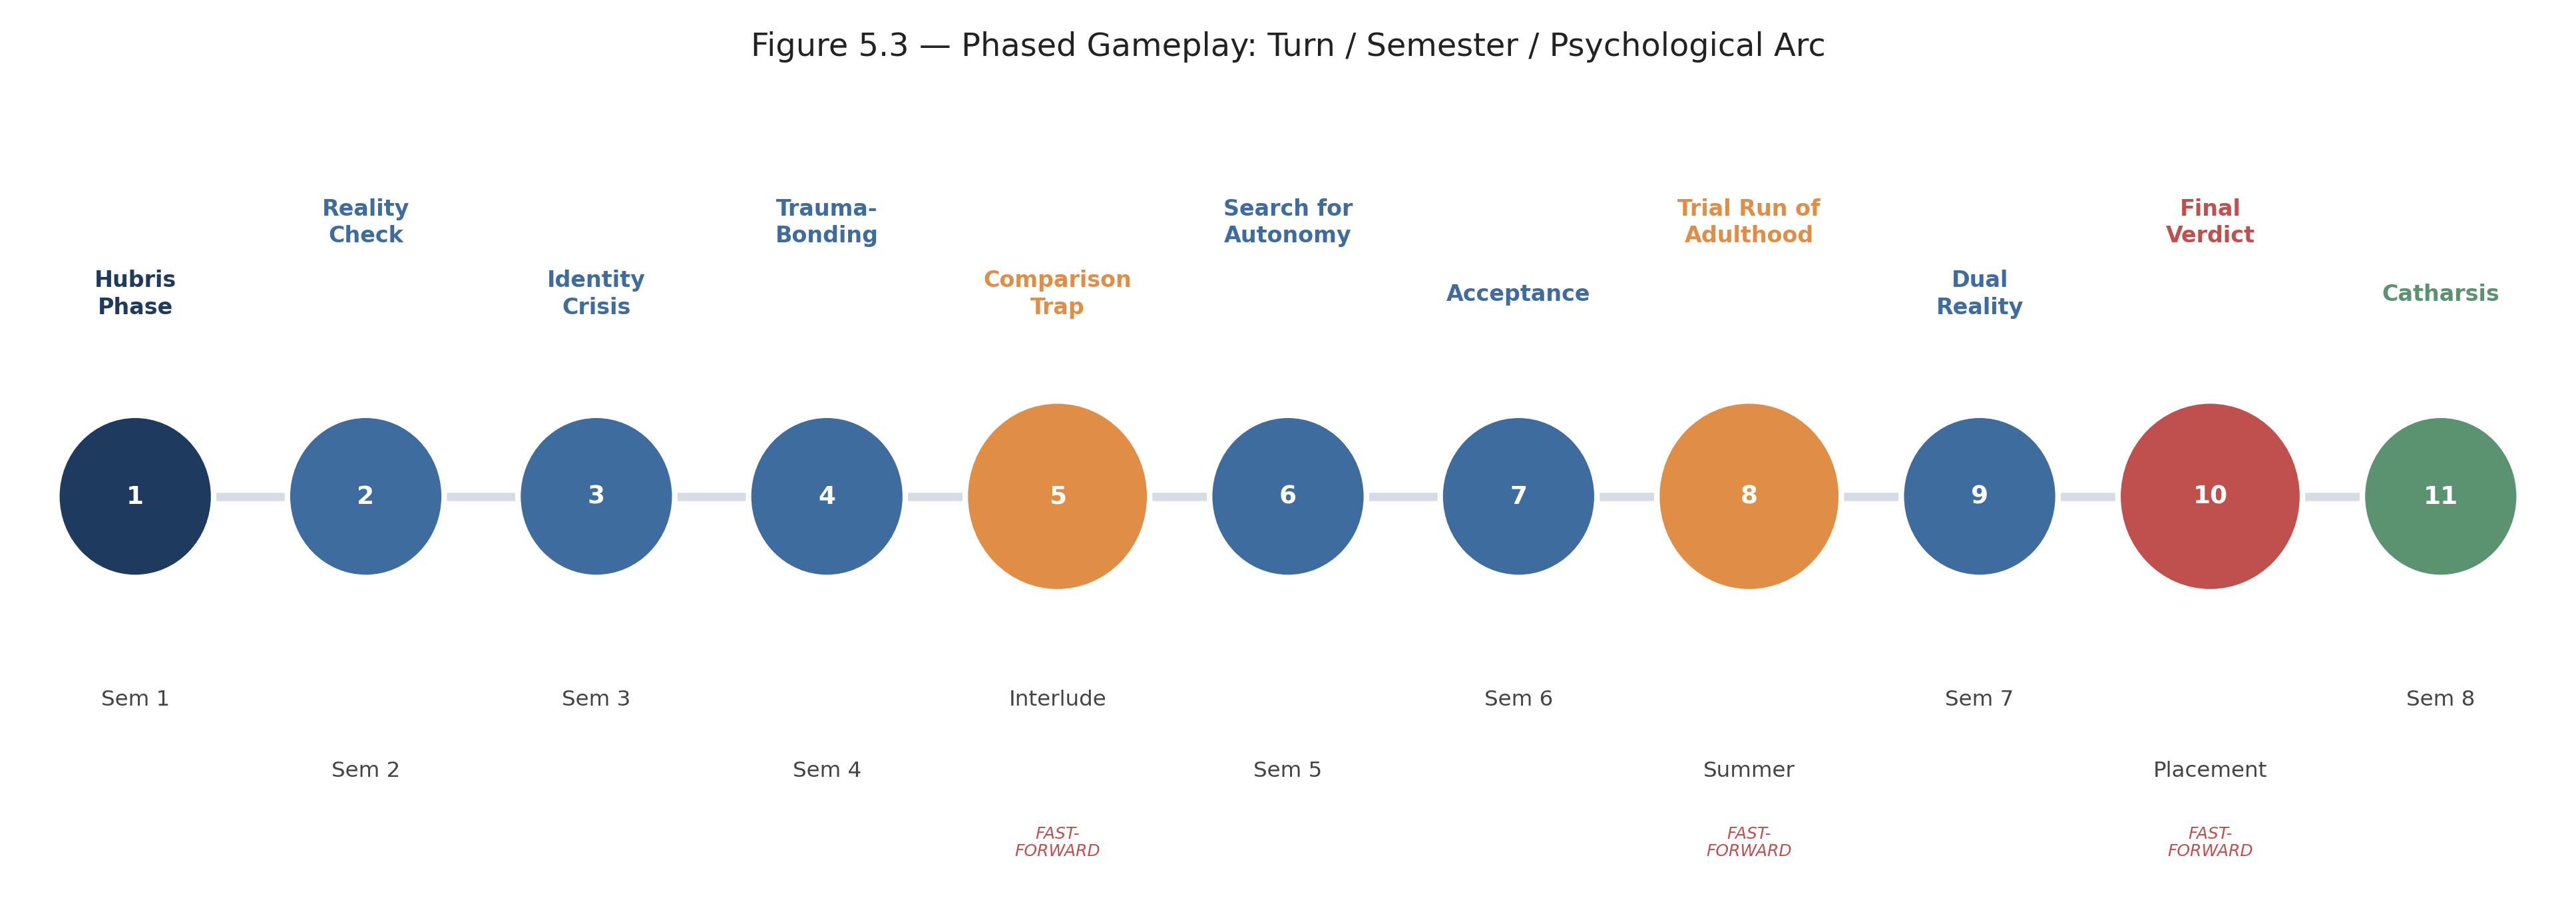
\includegraphics[width=0.8\textwidth]{Pictures/fig_5_1.png}
\caption{Figure 1 from Chapter 5}
\end{figure}

\emph{Figure 5.3 --- Phased Gameplay: Turn / Semester / Psychological Arc (from timeline.csv)}

The arc's own language is worth preserving directly: Semester 1 opens as \emph{"The Hubris Phase"} --- arriving "carrying the weight of being a topper" --- and by Semester 2 gives way to \emph{"Cognitive Dissonance"}, where, in the file's own words, \emph{"hard work does not guarantee an 'A' grade anymore."} This is not decorative flavor text sitting on top of the mechanics; it is the same design document as the mechanics --- the Reality Check phase (turn 2) is precisely when the SPI\emph{GRADING}SCALE first resolves a semester's Study investment into a number the player cannot argue with.

\subsection{Emergent Gameplay}

\begin{itemize}\item Compounding bad semesters: Stress from an unlucky Friction draw stacks with Stress from Debt Cascade (a Health or Money shortfall converting 1:1), which can trigger the Burnout Rule and block a planned high-value action --- a single rough week can cost a player more than the week itself.\item Track lock-in: POR tiers are both prerequisite-gated and semester-windowed (Sem\emph{End), so a track not started early enough cannot be caught up on later purely by spending more Time Blocks --- e.g. president}gymkhana (Sem_End = 8, requires the prior tier and Social $\geq$ 8) is simply unreachable for a player who starts the Gymkhana track in Semester 6.\item Divergent end-states from identical spend: because Study and resume stats (Algo/Res/Prod/POR) are earned from entirely non-overlapping cards, two players who spend the same total number of Time Blocks across the game can end up with completely different profiles --- one high-CPI/low-resume, one low-CPI/high-resume --- purely from allocation choices. Section 5.5 measures exactly how sharply this diverges.\item Emergent "home base" behavior: because Organic Social Encounters reward repeat visits to the same location rather than chasing novelty, players who lean into wellbeing tend to converge on 2--3 "home" locations rather than spreading visits thin --- an unplanned but thematically appropriate echo of Chapter 3's wing-centric reliance finding.\end{itemize}

\section{Playtesting}

\emph{This section has not been run yet --- it needs real 4-player sessions, not simulated ones. What follows is a ready-to-execute plan, not a report; replace the bracketed placeholders below with what actually happens once you run it.}

Recruitment: your Chapter 3 survey already produced a usable pool --- 58 of 113 respondents who answered the consent question (51.3\%) indicated willingness to be recontacted for playtesting. That is a large enough pool to comfortably fill 3--4 tables of 4 players each, drawn from a population that already understands the problem space the game addresses, without needing fresh recruitment.

\textbf{\emph{5.3.1 Methods Of Playtesting}}

\begin{itemize}\item Format: in-person, 4 players per table, matching the final product's player count exactly (a remote/digital playtest of the browser prototype could supplement this but should not replace an in-person physical-component test).\item Target: at minimum 2--3 full playthroughs (full 11-turn arc) with distinct groups, to separate genuine design issues from one group's idiosyncrasies.\item Instrumentation: a facilitator observation log (confusion points, house-ruling, turns where players stalled), a lightweight think-aloud prompt during the Placement turn specifically (since it is the highest-stakes single moment), and a short post-session questionnaire reusing a subset of your Chapter 3 Likert items (clarity, overwhelm, perceived fairness) so playtesting results are directly comparable to your survey baseline.\end{itemize}

\emph{\[ADD once run: exact dates, locations, number of sessions, and participant composition (Year/Branch mix, ideally including some of the same personas from Chapter 3.6).\]}

\textbf{\emph{5.3.2 Outcomes From Playtesting}}

\emph{\[ADD once run: what worked, what confused players, which mechanic needed the most facilitator intervention, and how session length compared to expectations.\]}

\textbf{\emph{5.3.3 Game Concept Tuning}}

\emph{\[ADD once run: concrete rule/number changes made in response to 5.3.2, with before/after values --- this is also where any Chapter 4 open decisions (Victory Conditions especially) should be confirmed against real player reactions rather than left as design-time proposals.\]}

\section{Final Product}

\subsection{Product Intro}

The final product is \emph{\[GAME NAME\]}, a 4-player physical board game adapting the validated digital economy described in Section 5.1 into a tabletop format. Every number quoted in this chapter --- Time Block costs, SPI thresholds, placement requirements --- carries forward unchanged from the working prototype; what remains to design is the physical form those numbers take.

\subsection{Game Components}

Proposed component list, derived directly from the CSV structure above (cross-check against your Chapter 4, Section 4.4.2 answer and reconcile any differences before finalizing):

\begin{itemize}\item 1 shared board --- 20 Action-phase locations (locations.csv), likely organized by Zone (Academic / Hostel / Social / Health / Career) rather than a linear path\item Project deck --- 9 cards\item POR deck --- 60 cards across 15 tracks (consider whether all 15 tracks belong in a physical deck, or whether a curated subset per playtest keeps table time reasonable --- flag as an open decision for 5.3.3)\item Internship deck --- 10 cards (7 SPO / 3 Off-Campus)\item Placement deck --- 8 cards, revealed only at the Placement turn\item Friction/Event deck --- 15 cards, shuffled and drawn once per turn\item Social/Network deck or tracker --- 8 contact cards, or a shared board track given they unlock deterministically rather than by draw\item 4 player mats --- tracking Health / Stress / Social / Money / Study / CPI / resume stats per player\item Time Block tokens (17 per player per semester) and resource tokens for the five survival stats\end{itemize}

\subsection{Game Board (4-Player Layout)}

\emph{\[Pending physical design --- headings ready to populate once you have a layout.\]}

\subsection{Player Mat / Character Sheet}

\emph{\[Pending physical design.\]}

\subsection{Cards}

\emph{\[Pending physical design --- content/values are already final (Section 5.1); this section needs visual/print design only.\]}

\subsection{Tokens}

\emph{\[Pending physical design.\]}

\subsection{Other Pieces}

\emph{\[Pending physical design.\]}

\subsection{Sequence Of Play}

A normal turn (1, 2, 3, 4, 6, 7, 9, 11) follows a fixed four-phase cycle:

\begin{itemize}\item 1\. Narrative --- the turn's phase and psychology are presented (Section 5.2.1); at turns 3, 6, and 9 the automatic Semester Recovery is also applied here.\item 2\. Friction --- one unavoidable random event is drawn and resolved (Section 5.1.8).\item 3\. Opportunity --- the player may draft one card from the Project, POR, or Off-Campus Internship pools available that semester (Sections 5.1.5--5.1.6).\item 4\. Action --- the player spends any remaining Time Blocks on locations (Section 5.1.4--5.1.5), each visit immediately ending the turn once resolved.\end{itemize}

Turns 5, 8, and 10 replace this cycle with a single narrative decision (Interlude internship shortlist, Summer path choice, Placement resolution) and allocate no ordinary Time Blocks. On academic turns, the Action phase closes with an SPI calculation and report-card reveal (Section 5.1.3) before advancing to the next turn's Narrative phase.

\subsection{Ending The Game}

The game concludes at turn 11 (Semester 8, "Catharsis") immediately following Placement resolution at turn 10. In the current single-player prototype, "ending" means the narrative closes and the best eligible offer (if any) is revealed. For the 4-player physical version, this is the point at which \textbf{Chapter 4's Victory Conditions} (Section 4.3.2) determine how the four players' final states are compared --- this section should be finalized once that decision is confirmed, rather than duplicated here.

\section{Balancing The Game Data}

Table 5.1 (Section 5.1.3) and Table 5.2 below give the core numeric benchmarks already encoded in GAME_CONFIG and the CSVs.

% Table row: | \textbf{Action Type}                                                 | \textbf{Typical Time Cost} | \textbf{Typical Reward}                        |
% Table row: | --------------------------------------------------------------- | --------------------- | ----------------------------------------- |
% Table row: | Academic location visit (LHC / NCL / Project Lab / Lab Session) | 1                     | +14 Study                                 |
% Table row: | Academic location visit (PKK Library)                           | 1 (+1 Study cost)     | +21 Study net +20                         |
% Table row: | Academic location visit (Core Dept Building, Sem 4+)            | 1                     | +21 Study                                 |
% Table row: | POR track, Tier 1 (Volunteer)                                   | 1                     | +0--1 POR                                  |
% Table row: | POR track, Tier 4 (Head / Fest Coordinator)                     | 4--5                   | +2--3 POR (+1 Prod, some tracks)           |
% Table row: | Project card                                                    | 2--5                   | +1--4 Algo / Res / Prod (varies)           |
% Table row: | Social maintenance (per contact, per semester)                  | 0--1                   | stat rewards + one-time career bonus      |
% Table row: | Random Friction event                                           | 0--1 (unavoidable)     | varies --- can be pure cost or pure benefit |

\emph{Table 5.2 --- Representative Time Block costs across systems}

\subsection{Simulated Playthroughs}

To check whether these numbers are balanced against each other, a Monte Carlo simulation was built in Python, re-implementing the exact formulas above (SPI\emph{GRADING}SCALE, the 17-block semester allowance, the Debt Cascade, the Burnout clamp, and the placement eligibility matching from Logic.evaluateAllPlacements) rather than estimating them. Five archetypal play strategies were run for 800 trials each: an \textbf{Academic Maximalist} (heavy Study focus), a \textbf{Balanced Builder} (even spread), a \textbf{POR Climber}, a \textbf{Portfolio Builder} (Project/Internship focus), and a \textbf{Low-Structure} archetype modelling the high-overwhelm, low-clarity behavior pattern from the Chapter 3.6 "Aditi" persona. This is a simplified proxy model --- one representative POR track, an approximated internship-eligibility flag, semesters 1--6 for the CPI lock and semester 7 for late resume-building --- built to check relative balance, not to predict exact play.

\begin{figure}[h]
\centering
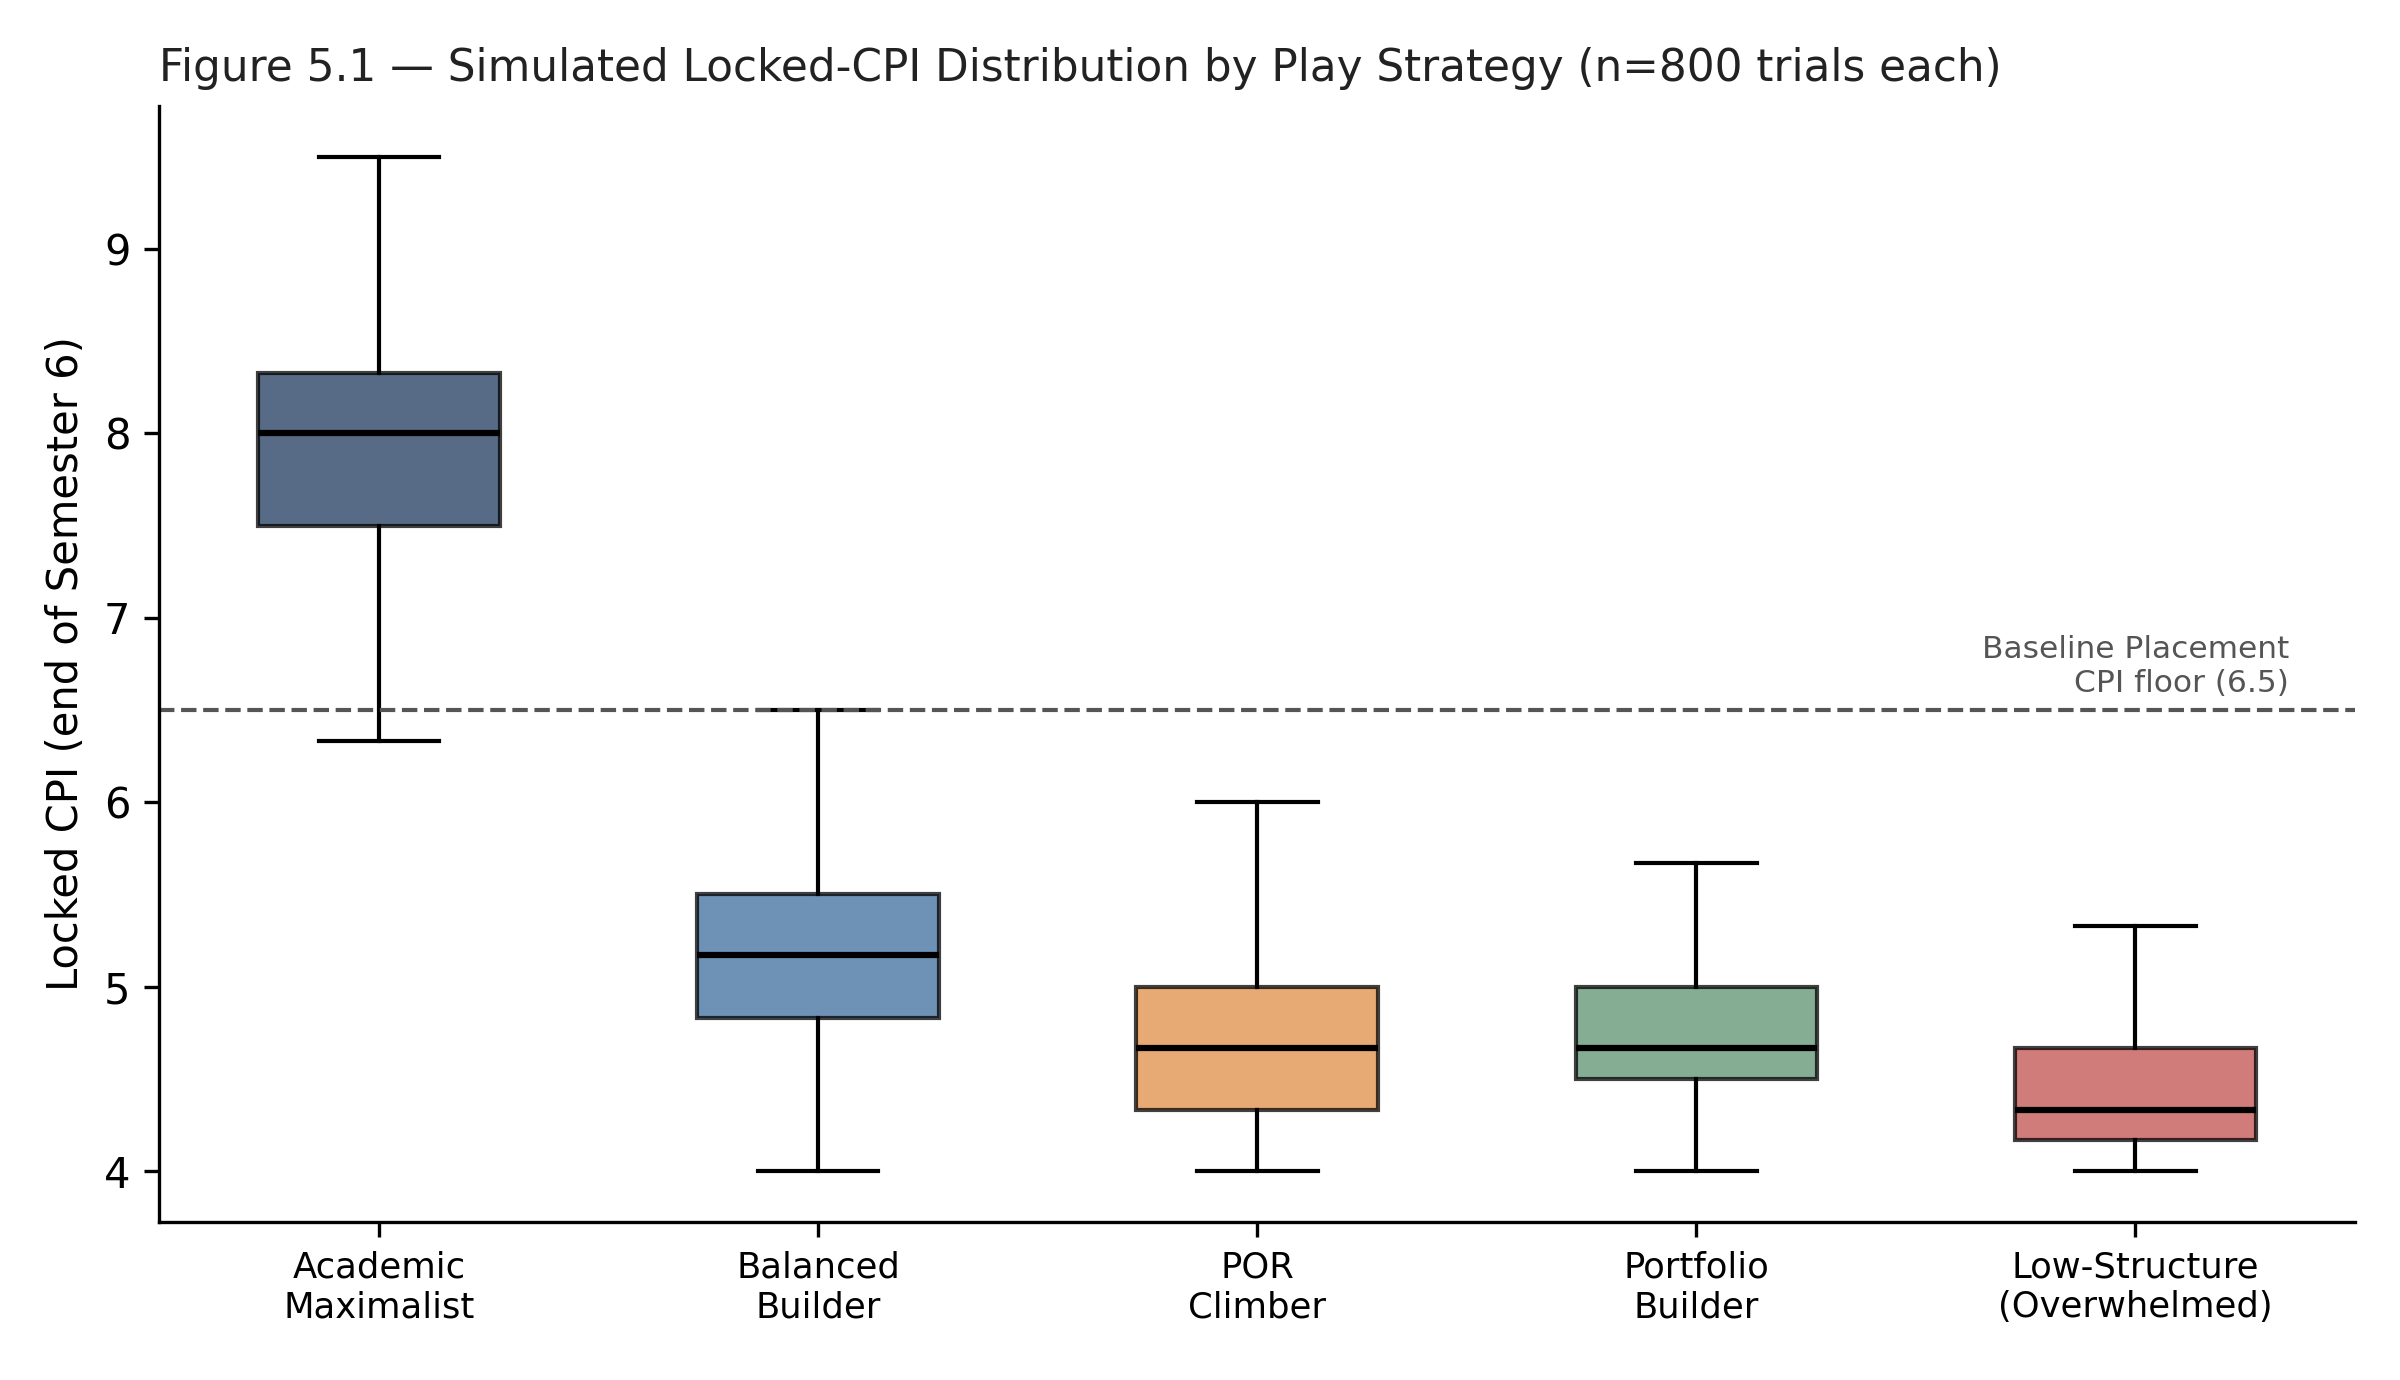
\includegraphics[width=0.8\textwidth]{Pictures/fig_5_2.png}
\caption{Figure 2 from Chapter 5}
\end{figure}

\emph{Figure 5.1 --- Simulated Locked-CPI Distribution by Play Strategy (n = 800 trials each)}

\begin{figure}[h]
\centering
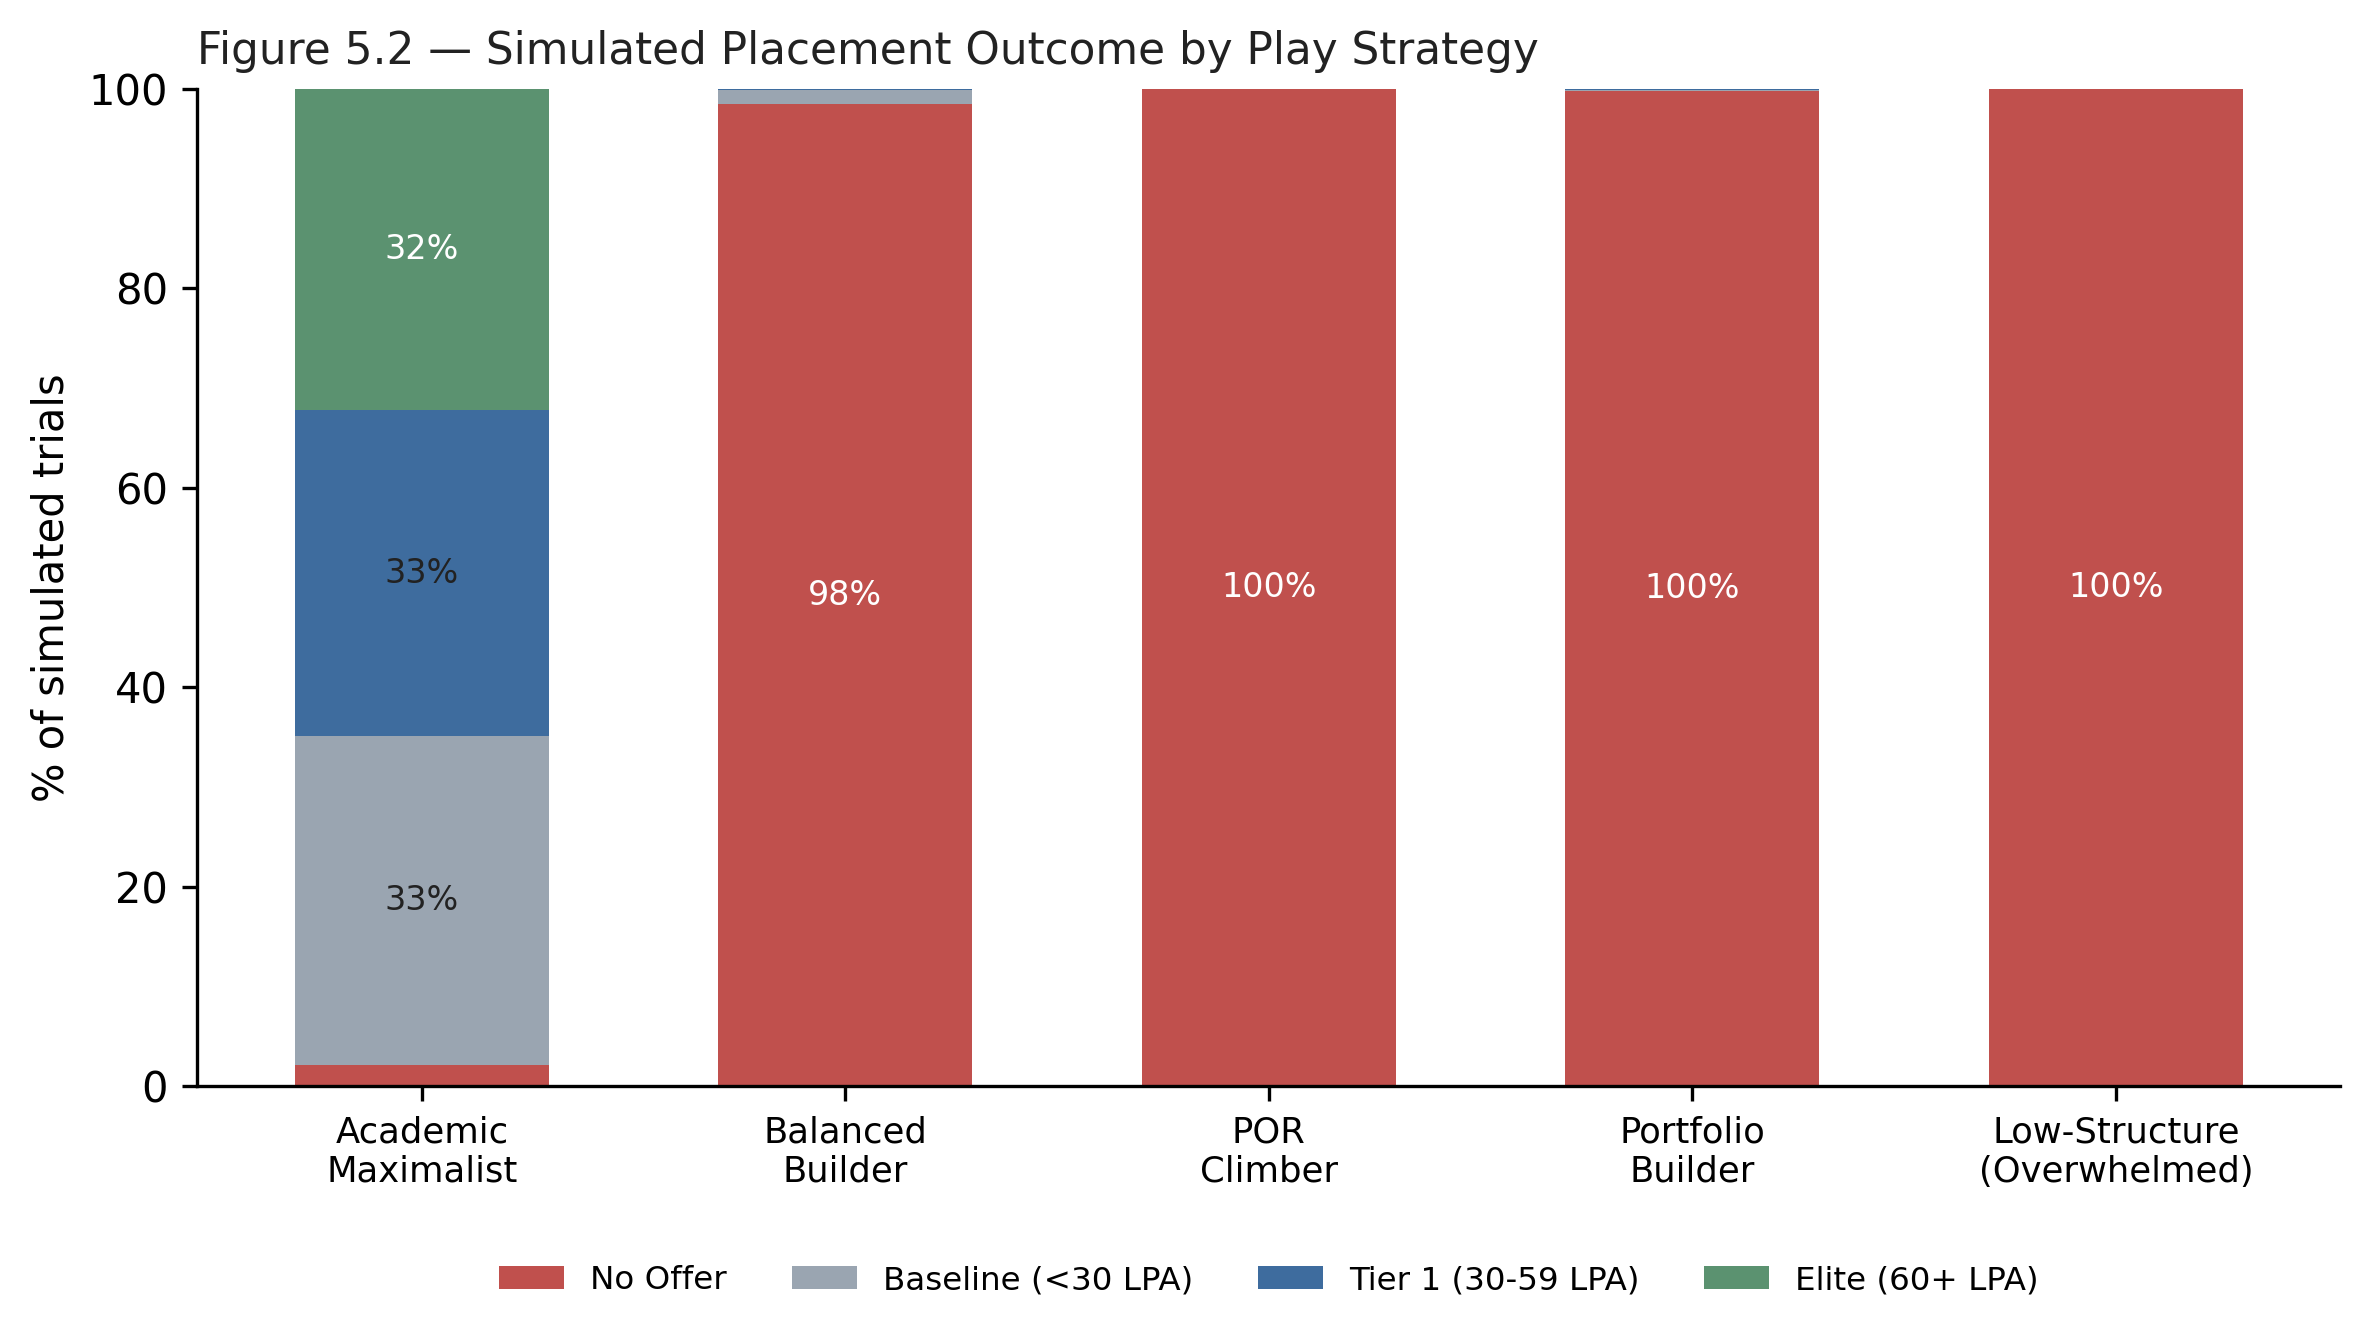
\includegraphics[width=0.8\textwidth]{Pictures/fig_5_3.png}
\caption{Figure 3 from Chapter 5}
\end{figure}

\emph{Figure 5.2 --- Simulated Placement Outcome by Play Strategy}

% Table row: | \textbf{Archetype}               | \textbf{Mean CPI} | \textbf{Median CPI} | \textbf{\% CPI$\geq$8.0} | \textbf{\% CPI<6.5} | \textbf{\% No Offer} | \textbf{Mean CTC (LPA)} |
% Table row: | --------------------------- | ------------ | -------------- | ------------- | ------------- | -------------- | ------------------ |
% Table row: | Academic Maximalist         | 7.92         | 8.00           | 53.1\%         | 1.1\%          | 2.1\%           | 49.4               |
% Table row: | Balanced Builder            | 5.20         | 5.17           | 0.0\%          | 98.5\%         | 98.5\%          | 0.3                |
% Table row: | POR Climber                 | 4.67         | 4.67           | 0.0\%          | 100.0\%        | 100.0\%         | 0.0                |
% Table row: | Portfolio Builder           | 4.75         | 4.67           | 0.0\%          | 99.8\%         | 99.8\%          | 0.1                |
% Table row: | Low-Structure (Overwhelmed) | 4.44         | 4.33           | 0.0\%          | 100.0\%        | 100.0\%         | 0.0                |

\emph{Table 5.3 --- Simulation summary across 5 archetypes Ã--- 800 trials}

\textbf{Finding.} Only the Academic Maximalist archetype reliably clears any placement gate (97.9\% receive an offer, mean CTC ≈₹49.4 LPA); all four other archetypes fail to reach even the Baseline Safe Placement CPI floor (6.5) in 98.5--100\% of trials, because Study --- and therefore SPI and CPI --- is earned exclusively from a small set of Academic locations, while Projects and PORs build entirely separate resume currencies that contribute nothing to CPI. As currently balanced, diversifying away from pure academic focus does not trade off against placement outcome --- it forfeits it almost entirely.

\textbf{This is worth a deliberate decision, not an accidental one.} Three directions are available: (a) lower the baseline CPI floor so a Balanced or Portfolio strategy can still clear it, (b) let select Projects or top-tier PORs grant a small Study side-reward so non-academic investment has some CPI payoff, or (c) keep the numbers as they are, treating the steep CPI gate as an intentional design statement --- a direct, playable echo of Chapter 3's own finding that IITK's system rewards academic focus far out of proportion to how much students say they value it (Section 3.3, Figure 3.11: Career Prep and Health \& Wellness are simultaneously the most wished-for and least-served domains). Whichever direction is chosen, it should be tested explicitly in Section 5.3 playtesting rather than decided from simulation data alone.

\textbf{This finding is not just a game-balance artifact --- it is independently supported by real data.} Section 3.8's decision-tree analysis of 57 real IITK resumes against their actual 2024 placement outcomes shows CPI and Algo_Rigor as the dominant splitting features across nearly every branch, with lower-CPI/lower-Algo profiles routed toward a narrower set of outcomes regardless of their POR, Research, or Product scores. The placement.csv thresholds this simulation tests were themselves informed by that same analysis (Section 3.8), so the sharp Academic-Maximalist-only result above is not an accident of arbitrary game numbers --- it is the game reproducing a pattern that is already present in real IITK placement data, which strengthens rather than undermines the case for treating it as a deliberate design statement (option (c) above).

\textbf{References}

This list consolidates all citations used across Chapters 1--5 into a single sequence. Reference \[43\] was added during the integration pass to correctly source the emerging-adulthood claim in Section 2.1, which previously pointed to an unrelated source (see the audit note at the end of this section).

\textbf{\[1\]} Lisa K. Simon. 2025. Is AI responsible for the rise in entry-level unemployment? Revelio Labs Macro News. Retrieved May 30, 2026 from <https://www.reveliolabs.com/news/macro/is-ai-responsible-for-the-rise-in-entry-level-unemployment/>

\textbf{\[2\]} Theodore Gerard Lynn, Pierangelo Rosati, Edel Conway, and Lisa van der Werff. 2023. The Future of Work: Challenges and Prospects for Organisations, Jobs and Workers. Palgrave Macmillan, Cham, Switzerland. <https://doi.org/10.1007/978-3-031-31494-0>

\textbf{\[3\]} Observer Research Foundation. 2023. Young India and Work: A Survey of Youth Aspirations. ORF Report. Retrieved May 30, 2026 from <https://www.orfonline.org/public/uploads/posts/pdf/20230420163450.pdf>

\textbf{\[4\]} Mercer Mettl. 2025. India's Graduate Skill Index 2025: Talent Readiness of Indian Graduates for an AI-Enabled Workplace. Technical Report. Retrieved May 30, 2026 from <https://www.mercer.com/insights/talent-and-transformation/talent-assessment/indias-graduate-skill-index-2025/>

\textbf{\[5\]} Gakujo Co., Ltd. 2023. Perspectives on Job Hunting: Survey of 2024 Graduates. PR TIMES Research Report. Retrieved May 30, 2026 from <https://service.gakujo.ne.jp/press/230412>

\textbf{\[6\]} Cabinet Office, Government of Japan. 2024. Survey on Student Job-Hunting Schedules and Academic Impact. Cabinet Office Economic and Social Research Institute Report. Retrieved May 30, 2026 from <https://www5.cao.go.jp/keizai1/gakuseichosa/index.html>

\textbf{\[7\]} Ziyi Wang, Ziwen Zeng, Yuan Li, and Zijian Ding. 2025. CareerPooler: AI-Powered Metaphorical Pool Simulation Improves Experience and Outcomes in Career Exploration. arXiv preprint arXiv:2509.11461. <https://doi.org/10.48550/arXiv.2509.11461>

\textbf{\[8\]} Koji Yatani, Zefan Sramek, and Chi-Lan Yang. 2024. AI as Extraherics: Fostering Higher-order Thinking Skills in Human-AI Interaction. arXiv preprint arXiv:2409.09218. <https://doi.org/10.48550/arXiv.2409.09218>

\textbf{\[9\]} Hayeon Jeon, Suhwoo Yoon, Keyeun Lee, et al. 2025. Letters from Future Self: Augmenting the Letter-Exchange Exercise with LLM-based Agents to Enhance Young Adults' Career Exploration. In Proceedings of the 2025 CHI Conference on Human Factors in Computing Systems (CHI '25). ACM, New York, NY, USA, 1--21. <https://doi.org/10.1145/3706598.3714206>

\textbf{\[10\]} Wantong Du, Zhiying Zhu, Xinhui Xu, Haoyuan Che, and Shi Chen. 2024. CareerSim: Gamification Design Leveraging LLMs For Career Development Reflection. In Extended Abstracts of the CHI Conference on Human Factors in Computing Systems (CHI EA '24). ACM, New York, NY, USA, 1--7. <https://doi.org/10.1145/3613905.3650928>

\textbf{\[11\]} Pat Pataranutaporn, Kavin Winson, Peggy Yin, Auttasak Lapapirojn, Pichayoot Ouppaphan, Monchai Lertsutthiwong, Pattie Maes, and Hal Hershfield. 2024. Future You: A Conversation with an AI-Generated Future Self Reduces Anxiety, Negative Emotions, and Increases Future Self-Continuity. arXiv preprint arXiv:2405.12514. <https://doi.org/10.48550/arXiv.2405.12514>

\textbf{\[12\]} Lisa A. Pace, Carmen Bruno, and Jan Oliver Schwarz. 2025. Personas in Scenario Building: Integrating Human-Centred Design Methods in Foresight. Futures 166 (February 2025), Article 103539. <https://doi.org/10.1016/j.futures.2025.103539>

\textbf{\[13\]} Brian J. Taber and Maureen Blankemeyer. 2015. Future Work Self and Career Adaptability in the Prediction of Proactive Career Behaviors. Journal of Vocational Behavior 86 (2015), 20--27.

\textbf{\[14\]} Danqi Wang and Yanling Li. 2024. Career Construction Theory: Tools, Interventions, and Future Trends. Frontiers in Psychology 15 (2024), Article 1381233.

\textbf{\[15\]} Bandura, A. 1986. Social Foundations of Thought and Action: A Social Cognitive Theory. Prentice-Hall.

\textbf{\[16\]} Hackett, G., \& Betz, N. E. 1981. A self-efficacy approach to the career development of women. Journal of Vocational Behavior, 18(3), 326--339. <https://doi.org/10.1016/0001-8791(81)90019-1>

\textbf{\[17\]} Savickas, M. L. 2013. Career construction theory and practice. In S. D. Brown \& R. W. Lent (Eds.), Career Development and Counseling (2nd ed., pp. 147--183). John Wiley \& Sons.

\textbf{\[18\]} Savickas, M. L., \& Porfeli, E. J. 2012. Career Adapt-Abilities Scale: Construction, reliability, and measurement equivalence across 13 countries. Journal of Vocational Behavior, 80(3), 661--673.

\textbf{\[19\]} Low, C. W., Cheng, M. Y., \& Ng, K. Y. 2026. Undergraduates' career adaptability: a systematic review of predictors, mediators, and outcomes. Issues and Perspectives in Business and Social Sciences, 6(2), 340--353. <https://doi.org/10.33093/ipbss.2026.6.2.8>

\textbf{\[20\]} Wang, Y. 2026. The impact of career adapt-abilities on AI anxiety among English majors: a dual perspective analysis based on core self-evaluations at the person- and variable-centered. Frontiers in Psychology, 17, Article 1767791. <https://doi.org/10.3389/fpsyg.2026.1767791>

\textbf{\[21\]} YaÅŸar, H., \& Karagucuk, V. 2025. The effect of artificial intelligence anxiety on career decidedness among students in English-related departments at universities. Discover Artificial Intelligence, 5(1), 48. <https://doi.org/10.1007/s44163-025-00284-y>

\textbf{\[22\]} Carkit, E. 2025. A social cognitive lens on employment anxiety and career optimism in the transition from school to work. The Career Development Quarterly, 73(3), 194--204. <https://doi.org/10.1002/cdq.70000>

\textbf{\[23\]} Zhang, J., Talib, M. A., \& Wang, J. 2025. Enhancing career adaptability and career decision-making self-efficacy through career planning education: a quasi-experimental study. Frontiers in Psychology, 16, 1612768. <https://doi.org/10.3389/fpsyg.2025.1612768>

\textbf{\[24\]} Maji, S., Chaturmohta, A., Deevela, D., Sinha, S., \& Barsaiya, A. 2024. Mental health consequences of academic stress, amotivation, and coaching experience: A study of India's top engineering undergraduates. Psychology in the Schools, 61(9), 3540--3566. <https://doi.org/10.1002/pits.23230>

\textbf{\[25\]} Afreen, \& Alam, S. 2022. Academic stress and suicidal ideation concerning mental health among coaching students preparing for technical entrance exams. International Journal of Multidisciplinary Educational Research, 11(11), 160--168.

\textbf{\[26\]} Chandrasekera, T., Hosseini, Z., Jayadas, A., \& Boorady, L. M. 2024. PeTe (Peer Teaching) Mentors: How Near Peer Mentoring (NPM) Affects Academic Success and Retention in Design Education. Innovative Higher Education, 49(5), 975--991. <https://doi.org/10.1007/s10755-024-09709-5>

\textbf{\[27\]} Yasar, D., \& Küçükali, U. F. 2026. Evaluating a near-peer mentoring model in a vertical studio: a mixed-methods case study with mentee and mentor perspectives. Cogent Education, 13(1), 2696606. <https://doi.org/10.1080/2331186X.2026.2696606>

\textbf{\[28\]} Bayeck, R. Y. 2020. Examining Board Gameplay and Learning: A Multidisciplinary Review of Recent Research. Simulation \& Gaming, 51(4), 411--431. <https://doi.org/10.1177/1046878119901286>

\textbf{\[29\]} Gee, J. P. 2007. What Video Games Have to Teach Us About Learning and Literacy (Revised ed.). Palgrave Macmillan.

\textbf{\[30\]} Gong, H., Bazakidi, E., \& Zary, N. 2019. Serious Games in Health Professions Education: Review of Trends and Learning Efficacy. Yearbook of Medical Informatics, 28(1), 240--248. <https://doi.org/10.1055/s-0039-1677904>

\textbf{\[31\]} Austad, A. F. 1988. Effects of peer mentoring on the achievement and persistence of academically underprepared college freshmen (Doctoral dissertation, University of the Pacific). <https://scholarlycommons.pacific.edu/uop_etds/504>

\textbf{\[32\]} Main, S., \& O'Rourke, J. 2011. 'New Directions for Traditional Lessons': Can Handheld Game Consoles Enhance Mental Mathematics Skills? Australian Journal of Teacher Education, 36(2), 43--55. <https://doi.org/10.14221/ajte.2011v36n2.4>

\textbf{\[33\]} Main, S., \& O'Rourke, J. 2017. Technology in the Classroom: Improving Automaticity in Mental-maths in Primary-aged Students. Australian Journal of Teacher Education, 42(10), 50--70. <https://doi.org/10.14221/ajte.2017v42n10.4>

\textbf{\[34\]} Sousa, M. 2021. City-building board games as systemic educational materials: an analysis of city-building board games. Urban Science, 5(3), 87. <https://doi.org/10.3390/urbansci5030087>

\textbf{\[35\]} Success Print Typographies \& Design Studio. 2024. Inspirational Board Game and Office Typographies. Etsy Shop Archive: Succation.

\textbf{\[36\]} Dhar, U., et al. 2022. Townshipâ„¢ as an empirical platform for resource scheduling. In Simulation and Gaming. ISAGA 2021, LNCS 13219, pp. 3--14. Springer. <https://doi.org/10.1007/978-3-031-09959-5_1>

\textbf{\[37\]} Bartolucci, M., Sparrow, L., \& Freeman, S. O. 2019. Tactile interaction and cognitive mapping in board game play. Journal of Educational Technology Systems, 48(1), 58--75. <https://doi.org/10.1177/0047239519854045>

\textbf{\[38\]} Booth, P. 2019. Board Gamers as Consumer-Fans: Sociality, Association, and Co-Presence in Analogue Play. Games and Culture, 16(2), 154--172. <https://doi.org/10.1177/1555412019890419>

\textbf{\[39\]} Pixelixe Design Blog. 2024. Exploring the role of print in modern digital design studios. Pixelixe Creatives.

\textbf{\[40\]} Carr, N. 2013, February 20. Students to e-textbooks: no thanks. Roughtype. <http://www.roughtype.com/?p=2922>

\textbf{\[41\]} Csikszentmihalyi, M. 1990. Flow: The Psychology of Optimal Experience. Harper \& Row.

\textbf{\[42\]} Malone, T. W. 1981. Toward a Theory of Intrinsically Motivating Instruction. Cognitive Science, 5(4), 333--369. <https://doi.org/10.1207/s15516709cog0504_2>

\textbf{\[43\]} Arnett, J. J. 2000. Emerging adulthood: A theory of development from the late teens through the twenties. American Psychologist, 55(5), 469--480. <https://doi.org/10.1037/0003-066X.55.5.469>

\emph{Integration-pass audit note: two citation errors were identified and corrected while assembling this consolidated list.}

\emph{(1) Section 2.1's opening sentence originally cited \[12, 13\] for "career agency represents an individual's capacity to direct their professional life" --- \[12\] (Pace, Bruno \& Schwarz, on persona-based foresight methodology) does not support this claim. The citation now reads \[13\] only.}

\emph{(2) The same section's emerging-adulthood claim ("ages 18--25... identity construction") originally cited \[9\] (Jeon et al., a CHI paper on LLM career-exploration agents) --- unrelated to the claim. It has been corrected to cite Arnett (2000), added here as \[43\].}

\emph{These were the two mismatches specifically identified during review. A full line-by-line audit of all 43 citations against their source papers has not been performed and is recommended before submission --- this pass fixed known errors, not all possible ones.}
 
%% Chapter Template

\chapter{Conclusions and Practical Implications}\doublespacing % Main chapter title

\label{Chapter6} % Change X to a consecutive number; for referencing this chapter elsewhere, use \ref{ChapterX}

\lhead{Chapter VI. \emph{Conclusions and Practical Implications}} % Change X to a consecutive number; this is for the header on each page - perhaps a shortened title

%----------------------------------------------------------------------------------------
%	SECTION 1
%----------------------------------------------------------------------------------------


\section{Summary}

This chapter outlines the findings and conclusions of the study, as well as the practical implications that can be drawn from the results.




\section{Study Findings}
\lipsum[1]

\begin{itemize}
    \item Urabitur auctor semper nulla. Donec varius orci eget risus. Duis nibh mi, congue eu, accumsan eleifend, sagittis quis, diam. Duis eget orci sit amet orci dignissim rutrum.

    \item Risus. Duis nibh mi, congue eu, accumsan eleifend, sagittis quis, diam.
\end{itemize}


\section{Research Contribution}
\lipsum[1]


\section{Practical Implications}
\lipsum[3]


\section{Study Limitations and Scope for Future Work}
\lipsum[3]



 

\clearpage 

%----------------------------------------------------------------------------------------
%	APPENDICES
%----------------------------------------------------------------------------------------

\addtocontents{toc}{\vspace{2em}} 

\appendix 

\input{Appendices/AppendixA}
\input{Appendices/AppendixB}

\addtocontents{toc}{\vspace{2em}} 

\backmatter

%----------------------------------------------------------------------------------------
%	BIBLIOGRAPHY
%----------------------------------------------------------------------------------------

\label{References}

\lhead{\emph{References}} 
\renewcommand\bibname{References}
\bibliographystyle{IEEEtran} 

\bibliography{references} 

%\newpage
%\include{LOP}
\newpage
\include{Biography}

\end{document}